% !TEX TS-program = XeLaTeX
% use the following command:
% all document files must be coded in UTF-8
\documentclass[portuguese]{textolivre}
% build HTML with: make4ht -e build.lua -c textolivre.cfg -x -u article "fn-in,svg,pic-align"


\journalname{Texto Livre}
\thevolume{19}
%\thenumber{1} % old template
\theyear{2026}
\receiveddate{\DTMdisplaydate{2025}{11}{28}{-1}} % YYYY MM DD
\accepteddate{\DTMdisplaydate{2026}{3}{9}{-1}}
\publisheddate{\DTMdisplaydate{2026}{3}{18}{-1}}
\corrauthor{Juliana Almansa Malagoli}
\articledoi{10.1590/1983-3652.2026.63121}
%\articleid{NNNN} % if the article ID is not the last 5 numbers of its DOI, provide it using \articleid{} commmand 
% list of available sesscions in the journal: articles, dossier, reports, essays, reviews, interviews, editorial
\articlesessionname{articles}
\runningauthor{Malagoli} 
%\editorname{Leonardo Araújo} % old template
\sectioneditorname{Daniervelin Pereira~\orcid{0000-0003-1861-3609}}
\layouteditorname{Leonardo Araújo~\orcid{0000-0003-3884-2177}}

\title{Robótica Pedagógica Livre: inovação no ensino de matemática e física na educação pública}
\othertitle{Open Pedagogical Robotics: innovation in mathematics and physics teaching in public education}
% if there is a third language title, add here:
%\othertitle{Artikelvorlage zur Einreichung beim Texto Livre Journal}

\author[1,2]{Juliana Almansa Malagoli~\orcid{0000-0002-8723-033X}\thanks{Email: \href{mailto:juliana.malagoli@ufpr.br}{juliana.malagoli@ufpr.br}}}
\affil[1]{Universidade Federal do Paraná, Pós-Graduação em Engenharia Elétrica, Curitiba, PR, Brasil.}
\affil[2]{Universidade Federal do Paraná, Centro de Estudos do Mar, Pontal do Paraná, PR, Brasil.}

%\usepackage{natbib}
%\usepackage[backend=biber,style=authoryear]{biblatex}
\addbibresource{article.bib}
% use biber instead of bibtex
%$ biber article

% used to create dummy text for the template file
\definecolor{dark-gray}{gray}{0.35} % color used to display dummy texts
\usepackage{lipsum}
\SetLipsumParListSurrounders{\colorlet{oldcolor}{.}\color{dark-gray}}{\color{oldcolor}}

% used here only to provide the XeLaTeX and BibTeX logos
\usepackage{hologo}

%\usepackage[colorlinks=true, linkcolor=blue, urlcolor=red]{hyperref}

% if you use multirows in a table, include the multirow package
\usepackage{multirow}

% provides sidewaysfigure environment
\usepackage{rotating}

% CUSTOM EPIGRAPH - BEGIN 
%%% https://tex.stackexchange.com/questions/193178/specific-epigraph-style
\usepackage{epigraph}
\renewcommand\textflush{flushright}
\makeatletter
\newlength\epitextskip
\pretocmd{\@epitext}{\em}{}{}
\apptocmd{\@epitext}{\em}{}{}
\patchcmd{\epigraph}{\@epitext{#1}\\}{\@epitext{#1}\\[\epitextskip]}{}{}
\makeatother
\setlength\epigraphrule{0pt}
\setlength\epitextskip{0.5ex}
\setlength\epigraphwidth{.7\textwidth}
% CUSTOM EPIGRAPH - END

% LANGUAGE - BEGIN
% ARABIC
% for languages that use special fonts, you must provide the typeface that will be used
% \setotherlanguage{arabic}
% \newfontfamily\arabicfont[Script=Arabic]{Amiri}
% \newfontfamily\arabicfontsf[Script=Arabic]{Amiri}
% \newfontfamily\arabicfonttt[Script=Arabic]{Amiri}
%
% in the article, to add arabic text use: \textlang{arabic}{ ... }
%
% RUSSIAN
% for russian text we also need to define fonts with support for Cyrillic script
% \usepackage{fontspec}
% \setotherlanguage{russian}
% \newfontfamily\cyrillicfont{Times New Roman}
% \newfontfamily\cyrillicfontsf{Times New Roman}[Script=Cyrillic]
% \newfontfamily\cyrillicfonttt{Times New Roman}[Script=Cyrillic]
%
% in the text use \begin{russian} ... \end{russian}
% LANGUAGE - END

% EMOJIS - BEGIN
% to use emoticons in your manuscript
% https://stackoverflow.com/questions/190145/how-to-insert-emoticons-in-latex/57076064
% using font Symbola, which has full support
% the font may be downloaded at:
% https://dn-works.com/ufas/
% add to preamble:
% \newfontfamily\Symbola{Symbola}
% in the text use:
% {\Symbola }
% EMOJIS - END

% LABEL REFERENCE TO DESCRIPTIVE LIST - BEGIN
% reference itens in a descriptive list using their labels instead of numbers
% insert the code below in the preambule:
%\makeatletter
%\let\orgdescriptionlabel\descriptionlabel
%\renewcommand*{\descriptionlabel}[1]{%
%  \let\orglabel\label
%  \let\label\@gobble
%  \phantomsection
%  \edef\@currentlabel{#1\unskip}%
%  \let\label\orglabel
%  \orgdescriptionlabel{#1}%
%}
%\makeatother
%
% in your document, use as illustraded here:
%\begin{description}
%  \item[first\label{itm1}] this is only an example;
%  % ...  add more items
%\end{description}
% LABEL REFERENCE TO DESCRIPTIVE LIST - END


% add line numbers for submission
%\usepackage{lineno}
%\linenumbers

\begin{document}
\maketitle

\begin{polyabstract}
\begin{abstract}
Este artigo apresenta uma proposta pedagógica que integra a robótica educacional ao ensino de matemática e física, utilizando tecnologias acessíveis e de baixo custo, adequadas à realidade da educação pública. O objetivo é oferecer um modelo replicável de atividade prática que favoreça a aprendizagem por experimentação e promova o protagonismo estudantil. Para isso, foi desenvolvido um sistema com arduino, sensores e visor, capaz de medir temperatura, umidade, distância e exibir os dados em tempo real. A partir desse protótipo, foram elaboradas atividades que permitem explorar termodinâmica, ondas sonoras, cinemática, movimento circular, funções, gráficos cartesianos, variação temporal, grandezas físicas e interpretação de dados. A metodologia fundamenta-se no construcionismo e na aprendizagem ativa, incentivando observar, criar, analisar e refletir. Além do potencial pedagógico, a proposta valoriza a reutilização de componentes eletrônicos e o uso de materiais livres, promovendo a consciência ambiental e a discussão sobre sustentabilidade. Os resultados indicam que a robótica, associada à sustentabilidade, favorece a construção do conhecimento, estimula a autonomia, o raciocínio lógico e aproxima teoria e prática de forma contextualizada. Portanto, é viável em escolas e universidades públicas, além de contribuir para uma educação científica, criativa, investigativa e ambientalmente responsável.

\keywords{Aprendizagem ativa \sep Construcionismo \sep Interdisciplinaridade \sep Robótica educacional}
\end{abstract}

\begin{english}
\begin{abstract}
This article presents a pedagogical proposal that integrates educational robotics into the teaching of mathematics and physics, using accessible and low-cost technologies suitable for the reality of public education. The objective is to offer a replicable model of practical activity that promotes learning through experimentation and encourages student protagonism. To this end, a system was developed using arduino, sensors, and a display, capable of measuring temperature, humidity, and distance, and displaying the data in real time. Based on this prototype, activities were designed to explore topics such as thermodynamics, sound waves, kinematics, circular motion, functions, cartesian graphs, temporal variation, physical quantities, and data interpretation. The methodology is grounded in constructionism and active learning, encouraging observation, creation, analysis, and reflection. In addition to its pedagogical potential, the proposal emphasizes the reuse of electronic components and the use of open-source materials, promoting environmental awareness and discussions about sustainability. The results indicate that robotics, combined with sustainability, supports knowledge construction, stimulates autonomy and logical reasoning, and connects theory and practice in a contextualized manner. Therefore, it is feasible in public schools and universities, in addition to contributing to a scientific, creative, investigative, and environmentally responsible education.

\keywords{Active learning \sep Constructionism \sep Interdisciplinarity \sep Educational robotics}
\end{abstract}
\end{english}
% if there is another abstract, insert it here using the same scheme
\end{polyabstract}

\section{Introdução}\label{sec-intro}

A educação pública brasileira enfrenta o desafio de integrar metodologias ativas e tecnologias digitais de forma crítica, criativa e acessível. Nesse contexto, a Robótica Educacional Livre surge como uma proposta inovadora capaz de promover o protagonismo estudantil, a aprendizagem significativa e a conscientização socioambiental. Dessa maneira, é fundamentada na filosofia do \textit{software} e \textit{hardware} livres, essa abordagem favorece a autonomia do educador e do estudante, permitindo a construção de soluções tecnológicas com materiais reutilizáveis e de baixo custo, uma prática essencial para o avanço da sustentabilidade no ambiente escolar \cite{linha,ultrassonico}.

De acordo com \textcite{ref0}, precursor do construcionismo, o aprendizado é potencializado quando o aluno participa ativamente da criação de objetos e experimentos que tenham significado pessoal. Essa concepção pedagógica inspira a aplicação da robótica no ensino de matemática e física, transformando conceitos abstratos em experiências concretas e contextualizadas.

Complementando a visão construcionista, \textcite{ref00} propõe a Espiral da Aprendizagem Criativa, um modelo que descreve o ciclo contínuo em que os aprendizes imaginam, criam, brincam, compartilham e refletem, aprimorando suas ideias e projetos a cada iteração (Figura \ref{fig_espiral}). Essa espiral representa o núcleo das práticas de aprendizagem criativa e colaborativa no uso da Robótica Educacional Livre, pois incentiva a curiosidade, o trabalho em equipe e a experimentação constante.

\begin{figure}[ht!]
	\centering
	\begin{minipage}{.43\textwidth}
        
\includegraphics[width=\textwidth]{figures/fig-001.jpg}
		\caption{Espiral da Aprendizagem Criativa.}
		\label{fig_espiral}
		\source{Adaptado de \textcite{ref00}.}
	\end{minipage}
\end{figure}

Além do desenvolvimento cognitivo e técnico, a robótica livre estimula a consciência ecológica e o pensamento sustentável, uma vez que incentiva o reaproveitamento de componentes eletrônicos, o uso racional de energia e a reflexão sobre o impacto ambiental das tecnologias. Essa perspectiva está em consonância com os Objetivos de Desenvolvimento Sustentável (ODS) da Agenda 2030 da Organização das Nações Unidas (ONU), especialmente o ODS 4 (Educação de Qualidade) e o ODS 7 (Energia Limpa e Acessível), reforçando o papel da escola pública como espaço de inovação social e científica \cite{ref0000}.

Segundo \textcite{ref000}, a inovação educacional exige práticas pedagógicas que unam tecnologia, sensibilidade humana e ética, favorecendo a formação de sujeitos criativos, críticos e solidários. Assim, ao integrar a Robótica Educacional Livre ao currículo escolar, especialmente nas áreas de matemática e física, promove-se não apenas o aprendizado técnico, mas também a valorização da sustentabilidade e da cidadania científica.

Dessa forma, este artigo tem como objetivo analisar o potencial da Robótica Educacional Livre como estratégia pedagógica inovadora para o ensino de matemática e física na educação pública, enfatizando sua contribuição para a consciência ambiental e para a formação de estudantes autônomos, críticos e criativos. 

Esta pesquisa possui abordagem qualitativa, de natureza aplicada, com objetivos exploratórios e descritivos. A pesquisa qualitativa busca compreender fenômenos educacionais a partir da interpretação das experiências e significados atribuídos pelos participantes ao processo de aprendizagem \cite{meto1}. Como estratégia metodológica, adotou-se a pesquisa-ação no contexto de um estudo de caso. Segundo \textcite{meto2}, a pesquisa-ação envolve a participação ativa dos sujeitos, visando compreender e transformar a realidade investigada. Nesse contexto, o estudo analisa experiências de aprendizagem com o uso da robótica pedagógica livre em atividades que integram conteúdos de física e matemática, fundamentadas em metodologias ativas e na abordagem STEAM (Ciência, Tecnologia, Engenharia, Artes e Matemática) \cite{ref3,ref4}.

Este trabalho foi dividido em seis seções: a \cref{sec-intro} descreve uma breve introdução do trabalho; a \cref{sec-historico} apresenta o contexto histórico da robótica educacional; na \cref{sec-robotica} relata sobre a robótica pedagógica livre; já na \cref{sec-metodologia} exibe as etapas desenvolvidas no trabalho; em sequência, a \cref{sec-resultados} evidencia os resultados do robô montado juntamente com as atividades criadas para aulas de robótica no ensino público; por fim, a \cref{sec-conclusoes} expõe as considerações finais do trabalho.

%\lipsum[1-5]

\section{Contexto histórico da robótica educacional}\label{sec-historico}

A trajetória da robótica educacional ao longo de cinco décadas é mostrada na Figura \ref{fig_linha}, de maneira objetiva e clara. Cada marco representa um passo importante: desde as primeiras pesquisas acadêmicas nos anos 1970, passando pelas ideias inovadoras de Papert e o uso dos robôs Turtle e LEGO/Logo nos anos 1980, até a chegada dos kits educacionais às escolas na década seguinte \cite{ref0,ref10}. Com o avanço das tecnologias e o acesso mais democrático a partir dos anos 2000, a robótica ganhou espaço como ferramenta de aprendizado criativa e interdisciplinar \cite{ref16}. Mais recentemente, em 2025, o foco se volta para os desafios e oportunidades trazidos por robôs sociais, inteligência artificial, inclusão e ética \cite{ref1,ref11,ref12}. Essa linha do tempo revela não apenas marcos históricos, mas também a evolução do pensamento educacional e tecnológico, mostrando como a robótica foi se transformando para atender diferentes contextos e gerações de estudantes.

\begin{figure}[htbp]
	\centering
	\begin{minipage}{.9\textwidth}
		
\includegraphics[width=\textwidth]{figures/fig-002.jpg}
		\caption{Linha do Tempo do surgimento da Robótica entre 1975 a 2025.}
		\label{fig_linha}
		\source{Autoria Própria.}
	\end{minipage}
\end{figure}

Desde suas origens, a robótica tem sido concebida como uma área voltada ao aprimoramento da vida humana. Em geral, as inovações tecnológicas emergem do desejo de oferecer soluções que ampliem as capacidades do ser humano e contribuam para o bem-estar coletivo. No caso dos sistemas robóticos, essa relação é ainda mais profunda, pois envolve não apenas a engenharia de máquinas, mas também reflexões éticas e filosóficas sobre o papel da tecnologia na sociedade.

O escritor e cientista Isaac Asimov foi um dos primeiros a explorar, de maneira sistemática, os dilemas éticos entre humanos e máquinas. Em sua obra \textit{I, Robot} \cite{ref15}, ele formulou as Três Leis da Robótica, posteriormente ampliadas para incluir a chamada Lei Zero \cite{ref16}. Essas leis orientam simbolicamente a interação entre seres humanos e robôs:
\begin{description}
    \item[Lei Zero:] Um robô não deve provocar qualquer dano à humanidade, nem permitir, por inação, que ela seja prejudicada.
    \item[Primeira Lei:] Um robô não pode produzir ferimento a um ser humano, nem permitir, por omissão, que um ser humano seja exposto a qualquer perigo.
    \item[Segunda Lei:] Um robô deve cumprir as ordens emitidas por seres humanos, exceto nos casos em que tais ordens contrariem a Primeira Lei.
    \item[Terceira Lei:] Um robô deve zelar por sua própria existência, desde que esse cuidado não entre em conflito com a Primeira ou a Segunda Lei.
\end{description}


Embora nascidas na ficção científica, essas diretrizes influenciaram profundamente o debate acadêmico e científico sobre ética em inteligência artificial, automação e robótica \cite{ref16}. Elas representam um ideal de responsabilidade moral que continua a inspirar pesquisadores e educadores no desenvolvimento de tecnologias seguras e socialmente conscientes.

Dessa maneira, a robótica educacional fundamenta-se nas teorias do construtivismo de Piaget, que vê o conhecimento como algo que o indivíduo constrói ativamente por meio da interação com o ambiente. Em 1980, essa teoria foi ampliada para o construcionismo de Papert, destacando que a aprendizagem é mais profunda quando os alunos constroem algo na prática, como robôs que funcionam em "micromundos" com elementos físicos e matemáticos \cite{ref0}. Nesse cenário, a utilização de robôs no ambiente escolar permite uma aprendizagem experimental e relevante, na qual teoria e prática se combinam.
 
Com o progresso da microeletrônica, da informática educacional e da oferta de kits robóticos acessíveis, iniciativas formais de robótica em instituições de ensino começaram a emergir nas décadas de 1980 e 1990. Por exemplo, plataformas como LEGO/Logo, os primeiros kits que uniam blocos físicos a sensores e atuadores controlados por lógica programável, permitiram que os docentes incorporassem a robótica como um elemento educacional nas aulas de matemática, ciências e tecnologia. Esse período marcou o início da utilização da robótica como ferramenta de ensino prático, com ênfase na lógica, na resolução de problemas e na integração de diferentes campos do conhecimento \cite{ref0,ref10}.

Na década de 2000, houve um aumento no número de programas e estudos em robótica educacional voltados para a democratização do acesso. As pesquisas começaram a investigar como a robótica pode ser incorporada ao currículo formal das escolas públicas, utilizando dispositivos de baixo custo, plataformas de código aberto e tecnologias que possibilitem adaptações locais \cite{ref17,ref16}. A educação digital também ganhou força, com políticas de inclusão digital, extensão universitária e capacitação direcionadas para que professores pudessem usar robótica em sala de aula.

A partir de meados da década de 2010, a robótica educacional começou a se incorporar de forma mais significativa à metodologia STEM (Ciência, Tecnologia, Engenharia e Matemática) e, em diversos casos, também ao STEAM, incluindo Artes. As pesquisas começaram a examinar não apenas o conteúdo técnico, mas também as habilidades socioemocionais, criatividade, pensamento crítico, persistência, colaboração e habilidade para resolver problemas complexos. Essa integração foi identificada em revisões sistemáticas, indicando que os programas de robótica na educação formal geram impactos positivos no conhecimento, nas atitudes e nas habilidades dos alunos \cite{ref16,ref4,ref3}.

O estudo bibliométrico intitulado "\textit{Robotics in Education: A Scientific Mapping of the Literature in Web of Science}" de \textcite{ref2} apresenta a evolução das pesquisas sobre robótica na educação de 1975 a 2019. Nesse estudo, os autores notam um crescimento irregular durante o período analisado, com um pico de produção no ano de 2019.   Eles também notam que a maioria dos artigos foi publicada nos anais de conferências e que as principais contribuições vieram de campos como engenharia, ciência da computação e educação. Os Estados Unidos se sobressaem como o país com o maior número de publicações. 

Um exemplo recente desse avanço é o estudo "\textit{Exploring the Features of Educational Robotics and STEM Research in Primary Education}" de \textcite{ref4}, que descreve intervenções robóticas no ensino fundamental, especificando tipos de desenho do estudo, equipamentos empregados, interfaces (tangíveis ou gráficas), duração das intervenções e objetivos das atividades. Eles enfatizam que muitos estudos têm duração e amostras pequenas, o que demanda a realização de intervenções mais longas e variadas.  

Uma contribuição mais recente é a meta-análise "The effects of educational robotics in STEM education: a multilevel meta-analysis" de \textcite{ref3}, que examinou estudos publicados de 2010 a 2022. A pesquisa revelou que a robótica educacional melhora o desempenho acadêmico e as atitudes dos estudantes. Esse estudo também indica fatores que influenciam esses efeitos, como a maneira de implementação, suporte ao docente e integração curricular. 

Em 2025, foram lançados capítulos e artigos que reexaminam a trajetória da robótica educacional, abordando aspectos como robôs sociais, robôs bioinspirados e novas plataformas de ensino. Por exemplo, o capítulo denominado "\textit{Educational Robots: Past, Present, Future}" de \textcite{ref1} revisita robôs educacionais iniciais, como a Turtle de Papert, além de discutir os desafios futuros relacionados ao uso de robôs com inteligência artificial nas instituições de ensino, abrangendo aspectos éticos, de acessibilidade e integração curricular. 

Há também um esforço acadêmico para tornar a robótica educacional mais inclusiva e adaptada a diferentes realidades escolares, desde escolas com muitos recursos até aquelas com recursos escassos, além de atender a diversas idades. As pesquisas recentes avaliam os pré-requisitos (desenvolvimento de competências e conhecimento prévio) necessários para que os estudantes possam aproveitar as intervenções em robótica educacional, especialmente na educação básica. 

Até 2025 a história da robótica educacional revela uma trajetória marcada por: (a) desenvolvimento teórico apoiado no construtivismo/construcionismo; (b) inovações tecnológicas que reduziram custo e aumentaram acessibilidade; (c) integração curricular e metodológica com STEM/STEAM; (d) crescente produção de pesquisa empírica e meta-análises demonstrando efeitos positivos; e (e) novos desafios quanto à duração das intervenções, escalabilidade, inclusividade, ética e uso de tecnologias mais avançadas como robôs sociais e inteligência artificial.

\section{Robótica Pedagógica Livre}\label{sec-robotica}

A robótica pedagógica livre emerge como uma proposta educacional transformadora, que vai além do simples uso de tecnologias em sala de aula. Ademais, é fundamentada no uso de \textit{software} e \textit{hardware} livres, ela se alinha às metodologias ativas e ao princípio de que os estudantes aprendem melhor quando atuam como protagonistas do próprio processo de construção do conhecimento.

O conceito de \textit{software} livre está fundamentado na ideia de que os usuários devem ter autonomia plena sobre os programas que utilizam. Isso significa que qualquer pessoa tem o direito de executar, estudar, modificar e compartilhar um \textit{software}, promovendo uma cultura de colaboração e aprendizado coletivo. De acordo com \textcite{ref17}, a liberdade do \textit{software} é expressa em quatro princípios fundamentais:
\begin{description}
    \item[Liberdade 0:] executar o programa para qualquer finalidade;
    \item[Liberdade 1:] estudar como o programa funciona e adaptá-lo às próprias necessidades;
    \item[Liberdade 2:] redistribuir cópias, contribuindo para que outras pessoas também se beneficiem;
    \item[Liberdade 3:] aprimorar o programa e compartilhar as melhorias com a comunidade.
\end{description}


Assim, o \textit{software} livre não representa apenas uma alternativa tecnológica, mas também um movimento que defende a democratização do saber e a independência digital. Em um contexto educacional, o uso de \textit{softwares} livres possibilita que professores e estudantes se tornem agentes ativos no processo de construção tecnológica, fortalecendo práticas pedagógicas baseadas na experimentação, na autonomia e na cooperação \cite{ref5}.

Dessa forma, na Figura \ref{fig_met} as metodologias ativas estão representadas como o núcleo central de um processo educacional dinâmico, no qual o aluno ocupa o papel de protagonista da aprendizagem e o professor atua como mediador e facilitador. Ao redor desse eixo central, destacam-se elementos fundamentais como reflexão, trabalho em equipe, aprendizagem baseada em problemas, inovação e autonomia, que se interligam para promover uma formação crítica, colaborativa e criativa. Assim, a robótica pedagógica incentiva o estudante a aprender de forma significativa, participativa e contextualizada, desenvolvendo competências essenciais para a resolução de problemas reais.

\begin{figure}[ht!]
	\centering
	\begin{minipage}{.65\textwidth}		
\includegraphics[width=\textwidth]{figures/fig-003.jpg}
		\caption{Metodologias ativas de aprendizagem.}
		\label{fig_met}
		\source{Autoria Própria.}
	\end{minipage}
\end{figure}

\newpage
De acordo com \textcite{ref0}, é inspirada no construcionismo, essa vertente da robótica educacional entende que a aprendizagem é mais profunda quando o aluno cria algo tangível, por exemplo, um robô, um protótipo, um programa e reflete sobre essa experiência. Papert destaca que “as crianças aprendem melhor quando estão ativamente envolvidas na construção de algo externo a elas, algo que possam compartilhar” \cite{ref0}. Esse “algo” pode ser tanto um objeto físico quanto um projeto coletivo que une ideias, experimentação e expressão pessoal.

Na escola, a robótica pedagógica livre estimula o desenvolvimento de competências cognitivas, sociais e emocionais, integrando o fazer com o pensar. Além disso, favorece o trabalho interdisciplinar e aproxima as áreas de ciência, tecnologia, engenharia, arte e matemática (STEAM), permitindo que os alunos compreendam conceitos abstratos por meio de experiências concretas.

Neste contexto, o uso de tecnologias abertas como o Arduino Nano e a Impressora 3D com material PLA (ácido polilático), democratiza o acesso à inovação, especialmente em escolas públicas e contextos com recursos limitados. Por serem ferramentas acessíveis e de código aberto, possibilitam que estudantes e professores compreendam os fundamentos da tecnologia, modifiquem e reinventem seus próprios dispositivos, fortalecendo a autonomia intelectual e a cultura da experimentação \cite{ref6}.

Como ressalta \textcite{ref7}, a robótica educacional deve ser compreendida como um ambiente de aprendizagem ativo, no qual o estudante aprende a compreender, explorando, testando hipóteses, errando e corrigindo seus próprios caminhos. Nessa perspectiva, a robótica pedagógica livre representa um espaço criativo para desenvolver o pensamento computacional, a inovação e a resolução de problemas, habilidades essenciais para a formação integral dos cidadãos do século XXI.

A seguir, são apresentadas duas ferramentas amplamente aplicadas: o Arduino Nano, voltado à experimentação e à aprendizagem ativa, e a Impressão 3D com PLA, que possibilita prototipagem sustentável e criativa no ambiente educacional.


\subsection{Arduino nano: aprendizagem ativa e formação tecnológica}

O Arduino Nano é um microcontrolador de código aberto que se tornou um símbolo da educação tecnológica contemporânea. Além disso, é compacto, versátil e de baixo custo, ele possibilita que alunos construam protótipos eletrônicos e robôs de maneira prática, conectando teoria e experiência de forma dinâmica \cite{arduino}. A Figura \ref{fig_arduino} mostra (a) uma imagem do arduino nano e (b) um desenho do arduino nano com destaque dos pinos. 

\begin{figure}[ht!]
	\begin{minipage}[t]{0.18\textwidth}
		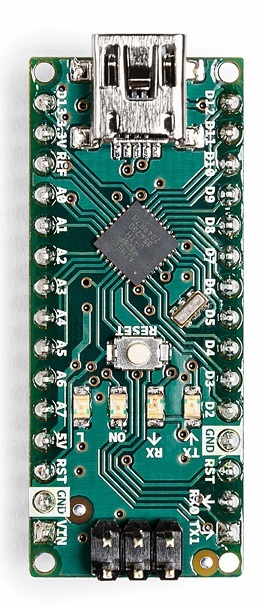
\includegraphics[width=\linewidth]{figures/fig-004a.jpg}
		\subcaption{Arduino nano.}
	\end{minipage}
	\hfill
	\begin{minipage}[t]{0.55\textwidth}
		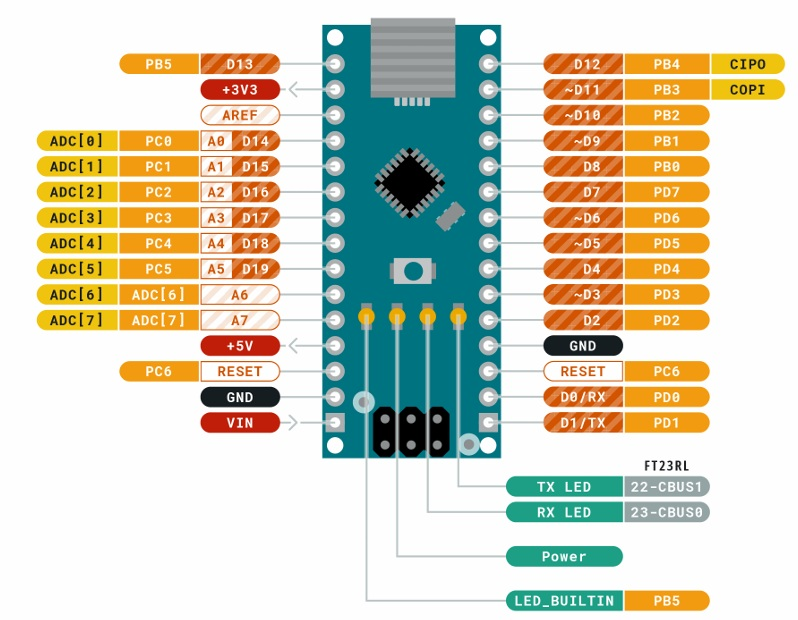
\includegraphics[width=\linewidth]{figures/fig-004b.jpg}
		\subcaption{Pinos do arduino nano.}
	\end{minipage}
	
	\caption{Detalhes do arduino nano.}
	\label{fig_arduino}
	\source{\textcite{arduino}}
\end{figure}

Em projetos pedagógicos, o uso do arduino permite aos estudantes aprenderem fazendo, um dos princípios centrais do construcionismo. Eles programam, testam sensores e atuadores, observam resultados e refletem sobre os processos, desenvolvendo o raciocínio lógico e a autonomia intelectual.

Do ponto de vista pedagógico, o Arduino Nano contribui para o fortalecimento do pensamento computacional, uma competência essencial para compreender e atuar no mundo digital. Por meio da robótica livre, os alunos não apenas aprendem a programar, mas também a planejar, projetar e solucionar problemas reais de forma criativa e colaborativa  \cite{wing}.

Além disso, o \textit{software} aberto do Arduino cria uma rede global de aprendizagem, onde professores e estudantes compartilham códigos, ideias e projetos, favorecendo o espírito comunitário e o aprendizado coletivo. Essa rede representa uma nova forma de alfabetização tecnológica, pautada pela ética do compartilhamento e pela coautoria do conhecimento \cite{ref17}.


\subsection{Impressão 3D e material PLA: prototipagem sustentável e criativa na educação}

A impressão 3D constitui uma das tecnologias mais inspiradoras para o ensino contemporâneo, por possibilitar que os estudantes transformem ideias em objetos concretos. No contexto da robótica pedagógica livre, ela amplia o alcance do aprendizado experimental, permitindo que os alunos projetem, modelem e fabriquem peças e estruturas personalizadas para seus robôs e dispositivos \cite{ref18}. A Figura \ref{fig_impresso} apresenta a impressora 3D usada neste trabalho e um exemplo de várias cores de filamento PLA.

\begin{figure}[ht!]
\centering
\begin{minipage}{0.7\textwidth}
	\begin{minipage}[t]{0.3\textwidth}
		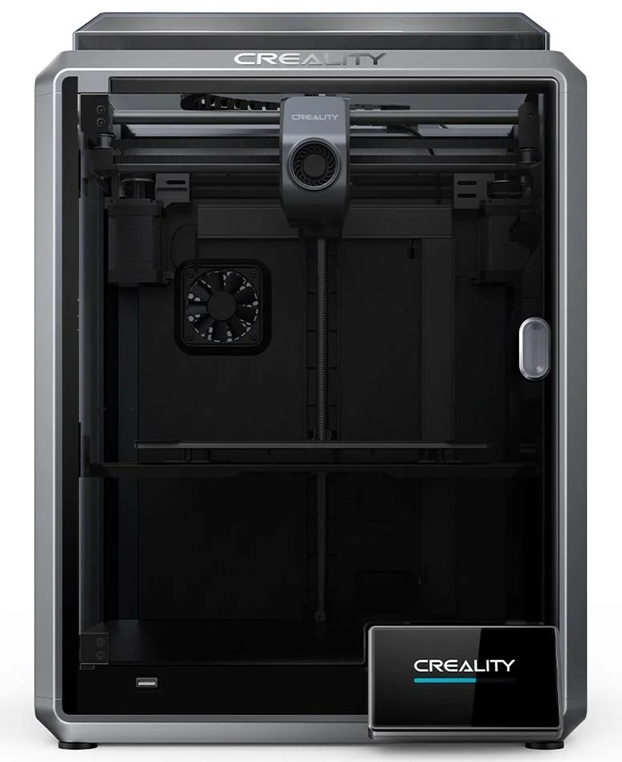
\includegraphics[width=\linewidth]{figures/fig-005a.jpg}
		\subcaption{Impressora 3D de modelo Creatily k1.}
	\end{minipage}
	\hspace{5em}
	\begin{minipage}[t]{0.4\textwidth}
		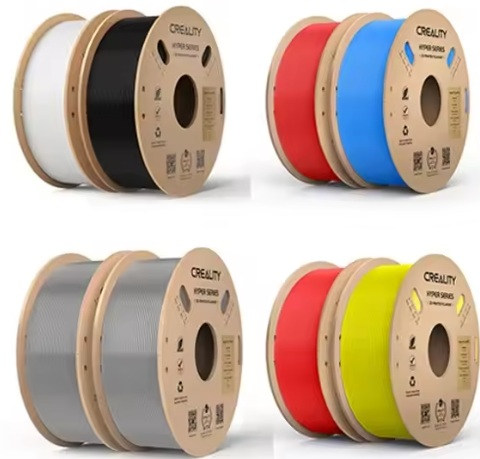
\includegraphics[width=\linewidth]{figures/fig-005b.jpg}
		\subcaption{Exemplo de várias cores de filamento PLA.}
	\end{minipage}
	
	\caption{Impressora 3D e Filamentos PLA.}
	\label{fig_impresso}
	\source{Autoria Própria.}
\end{minipage}
\end{figure}

Quando associada ao uso do material PLA (ácido polilático), um biopolímero biodegradável derivado de fontes renováveis como o milho e a cana-de-açúcar, a impressão 3D também assume um papel sustentável e ecológico dentro da educação tecnológica \cite{ref22}. Essa combinação permite abordar, de forma integrada, temas de ciência dos materiais, sustentabilidade e inovação, em consonância com os ODS da ONU, especialmente o ODS 9 (Indústria, Inovação e Infraestrutura) e o ODS 12 (Consumo e Produção Responsáveis). 

Do ponto de vista do ensino, a prototipagem em 3D promove o aprendizado baseado em projetos como PBL (\textit{Project Based Learning}), incentivando a resolução criativa de problemas reais. Os estudantes passam por todas as etapas do processo de projeto: concepção, modelagem, impressão e montagem, ao longo desse percurso, desenvolvem competências como planejamento, pensamento espacial, raciocínio científico e cooperação \cite{ref19,ref20,ref21}.

A robótica educacional é uma prática que integra o fazer e o pensar, e a impressão 3D representa a materialização dessa integração, tornando o aprendizado mais tangível, expressivo e socialmente relevante. A prototipagem 3D também favorece a experimentação iterativa: erros e ajustes fazem parte do processo, incentivando o pensamento crítico e a capacidade de resolver problemas de maneira criativa \cite{ref24}. Assim, a combinação de Arduino Nano e impressão 3D não apenas introduz conceitos tecnológicos, mas cria um ambiente educativo rico para o desenvolvimento de habilidades técnicas, cognitivas e socioemocionais.

\section{Metodologia na construção do robô}\label{sec-metodologia}

Esta pesquisa caracteriza-se como qualitativa, de natureza aplicada, com objetivos exploratórios e descritivos, e adota como procedimento metodológico a pesquisa-ação (estudo de caso). A escolha dessa abordagem justifica-se por buscar compreender, em profundidade, as experiências de aprendizagem proporcionadas pela utilização da robótica pedagógica livre, especialmente com o robô, em atividades que integram conteúdos de física e matemática. Assim, o estudo visa não apenas analisar, mas também intervir no processo educativo, promovendo práticas baseadas em metodologias ativas e princípios STEAM (Ciência, Tecnologia, Engenharia, Artes e Matemática).

O processo metodológico foi dividido em três etapas: construção da estrutura do robô, desenvolvimento do circuito eletrônico e código-fonte aberto. Cada etapa foi planejada de forma a garantir a integração entre teoria e prática, favorecendo a aprendizagem significativa e o desenvolvimento de competências investigativas e tecnológicas.

A Figura \ref{fig_fluxo} apresenta uma visão geral do percurso metodológico adotado neste estudo, que foi estruturado em quatro etapas principais: estrutura do robô, circuito eletrônico, código-fonte e aplicação das atividades pedagógicas. Essa organização busca evidenciar o processo integrado de desenvolvimento do projeto, desde a construção física e eletrônica do robô até sua utilização em práticas educativas interdisciplinares.

\begin{figure}[ht!]
	\centering
	\begin{minipage}{.85\textwidth}		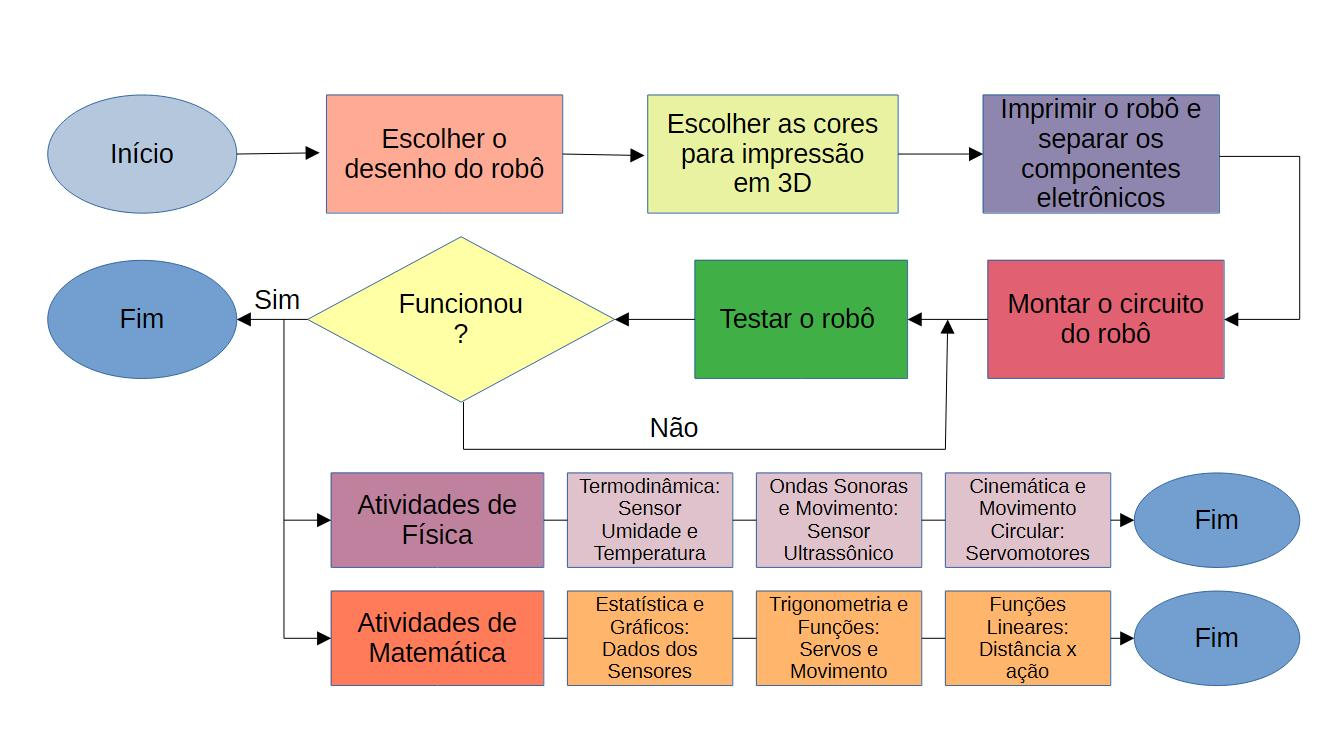
\includegraphics[width=\textwidth]{figures/fig-006.jpg}
		\caption{Fluxograma das etapas do trabalho.}
		\label{fig_fluxo}
		\source{Autoria Própria.}
	\end{minipage}
\end{figure}

O fluxograma ilustra a sequência lógica das ações realizadas, destacando a natureza iterativa e colaborativa da pesquisa, em consonância com os princípios da pesquisa-ação e das metodologias ativas. Essa estrutura metodológica favorece a articulação entre a teoria e a prática, permitindo que o robô se torne um recurso de experimentação para os conceitos de física e matemática no ensino público.

\subsection{Estrutura do robô}

O robô foi construído a partir de peças impressas em 3D, utilizando o material PLA (ácido polilático), devido à sua leveza, resistência e baixo custo, características que o tornam ideal para projetos pedagógicos. As peças foram projetadas para acomodar todos os componentes eletrônicos e proporcionar liberdade de movimento aos servomotores, mantendo estabilidade durante o deslocamento.

O processo de impressão 3D foi dividido em etapas de modelagem, fatiamento, impressão e montagem, com ajustes finos para garantir encaixes precisos e resistência mecânica nas articulações. A estrutura física do robô é formada por quatro partes principais: pés, pernas, corpo e cabeça (Figura \ref{estrutura}). Além disso, os componentes eletrônicos são ilustrados na Figura \ref{eletronica}.

\begin{figure}[ht!]
	\centering	\begin{minipage}{.65\textwidth}		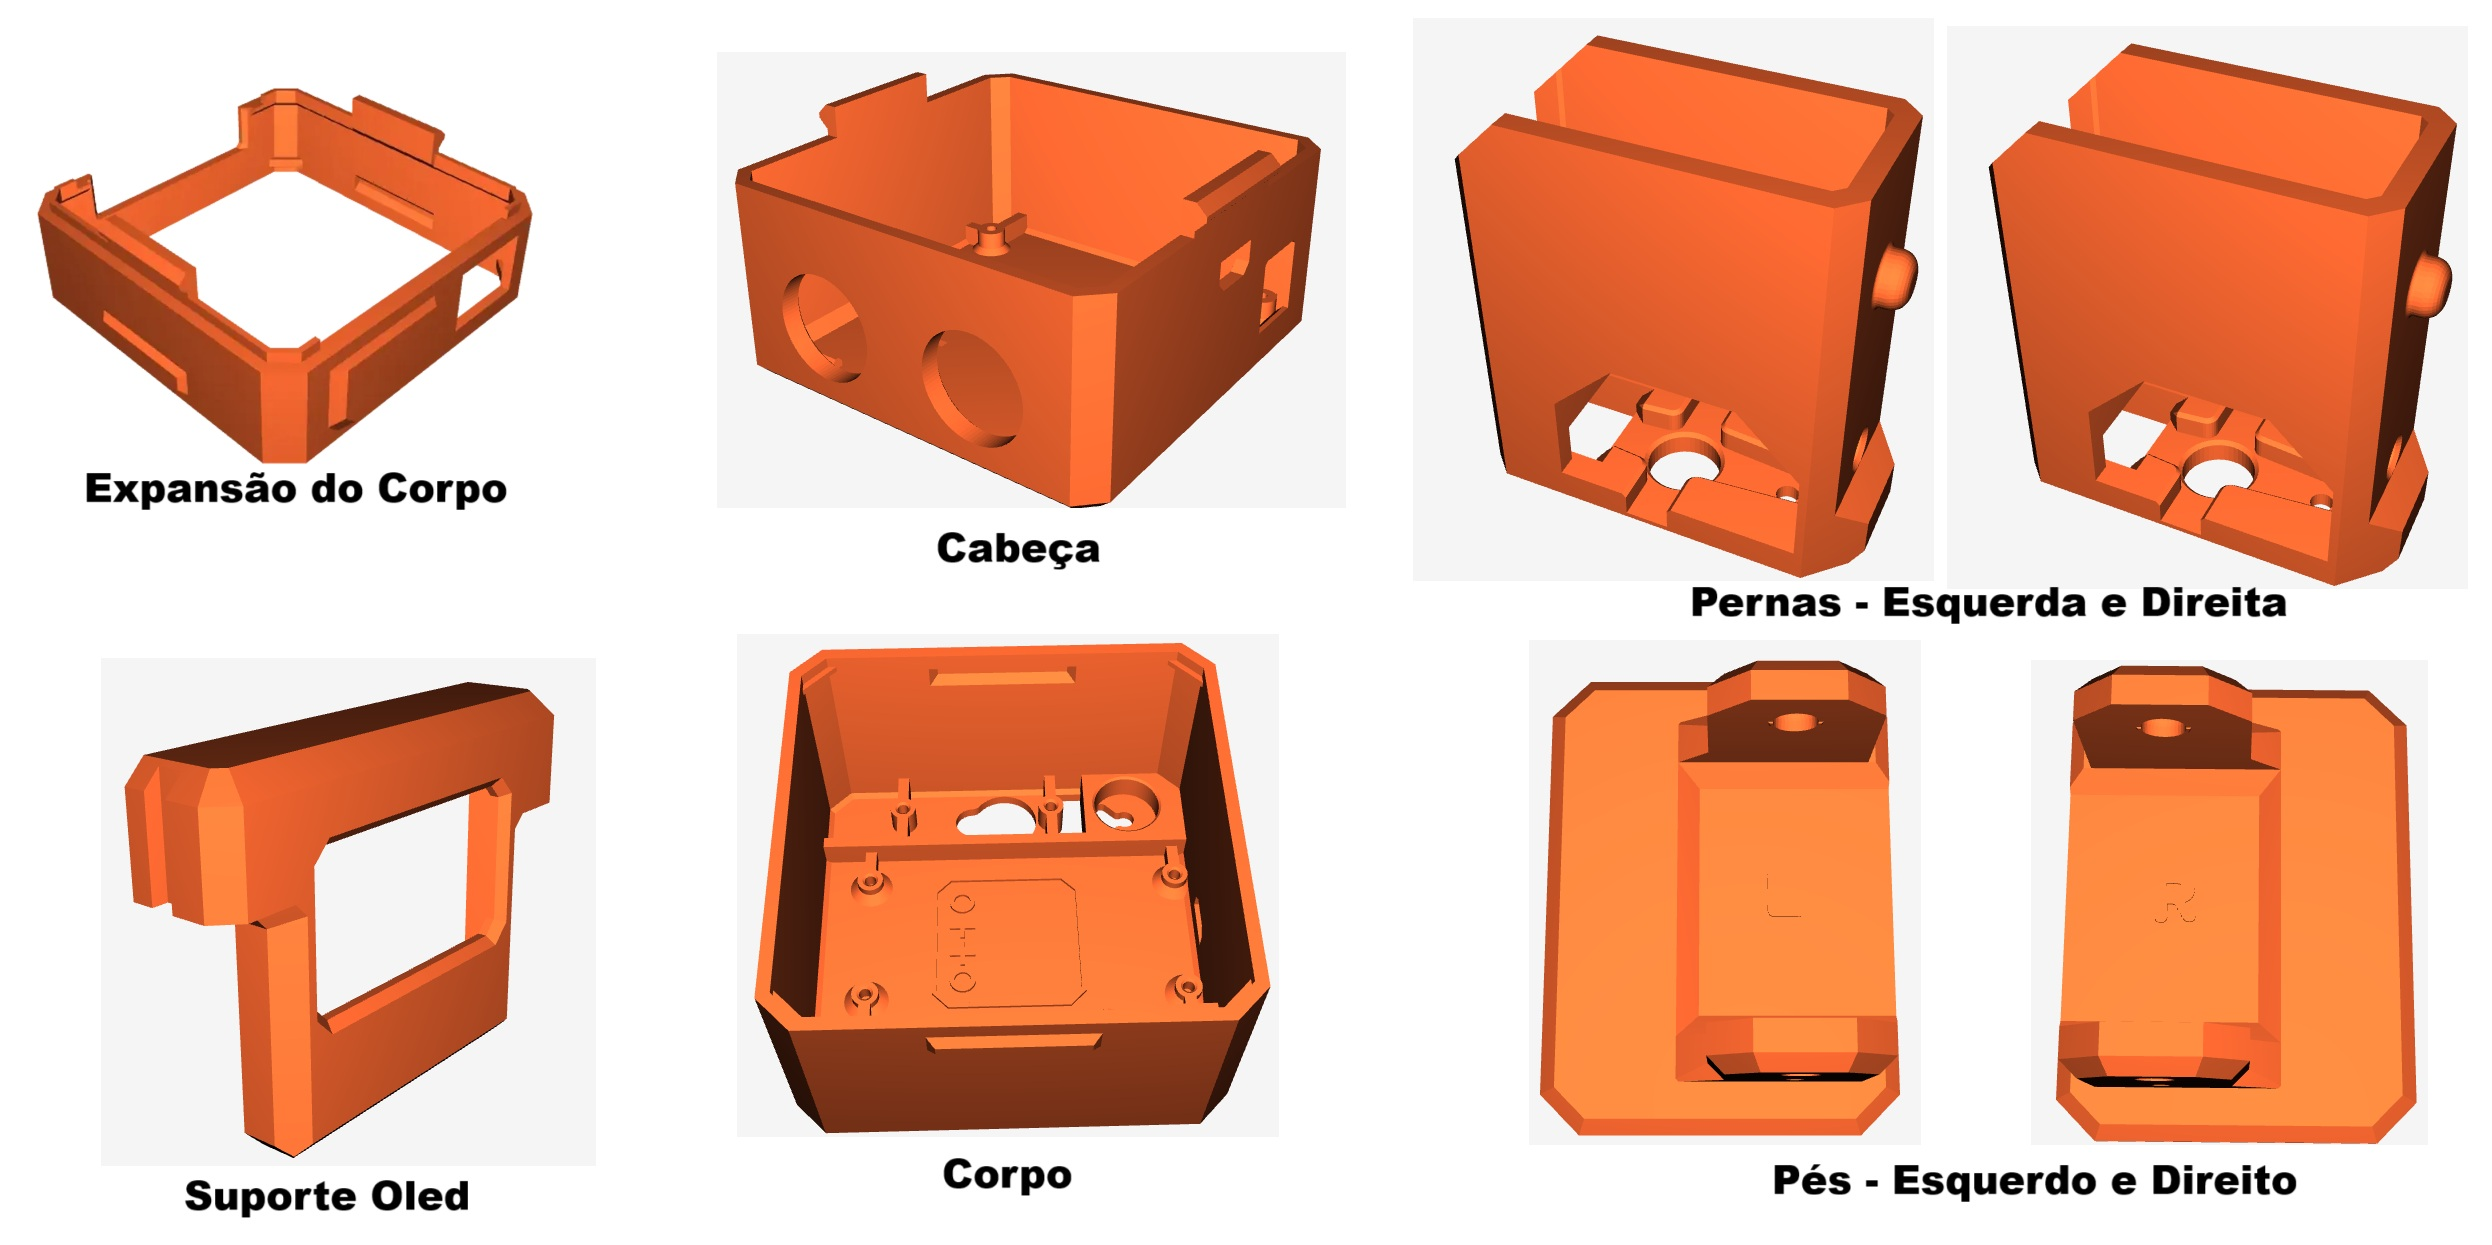
\includegraphics[width=\textwidth]{figures/fig-007.jpg}
		\caption{Estruturas das peças.}
		\label{estrutura}
		\source{Autoria Própria.}
	\end{minipage}
\end{figure}

\begin{figure}[ht!]
	\centering
	\begin{minipage}{.9\textwidth}		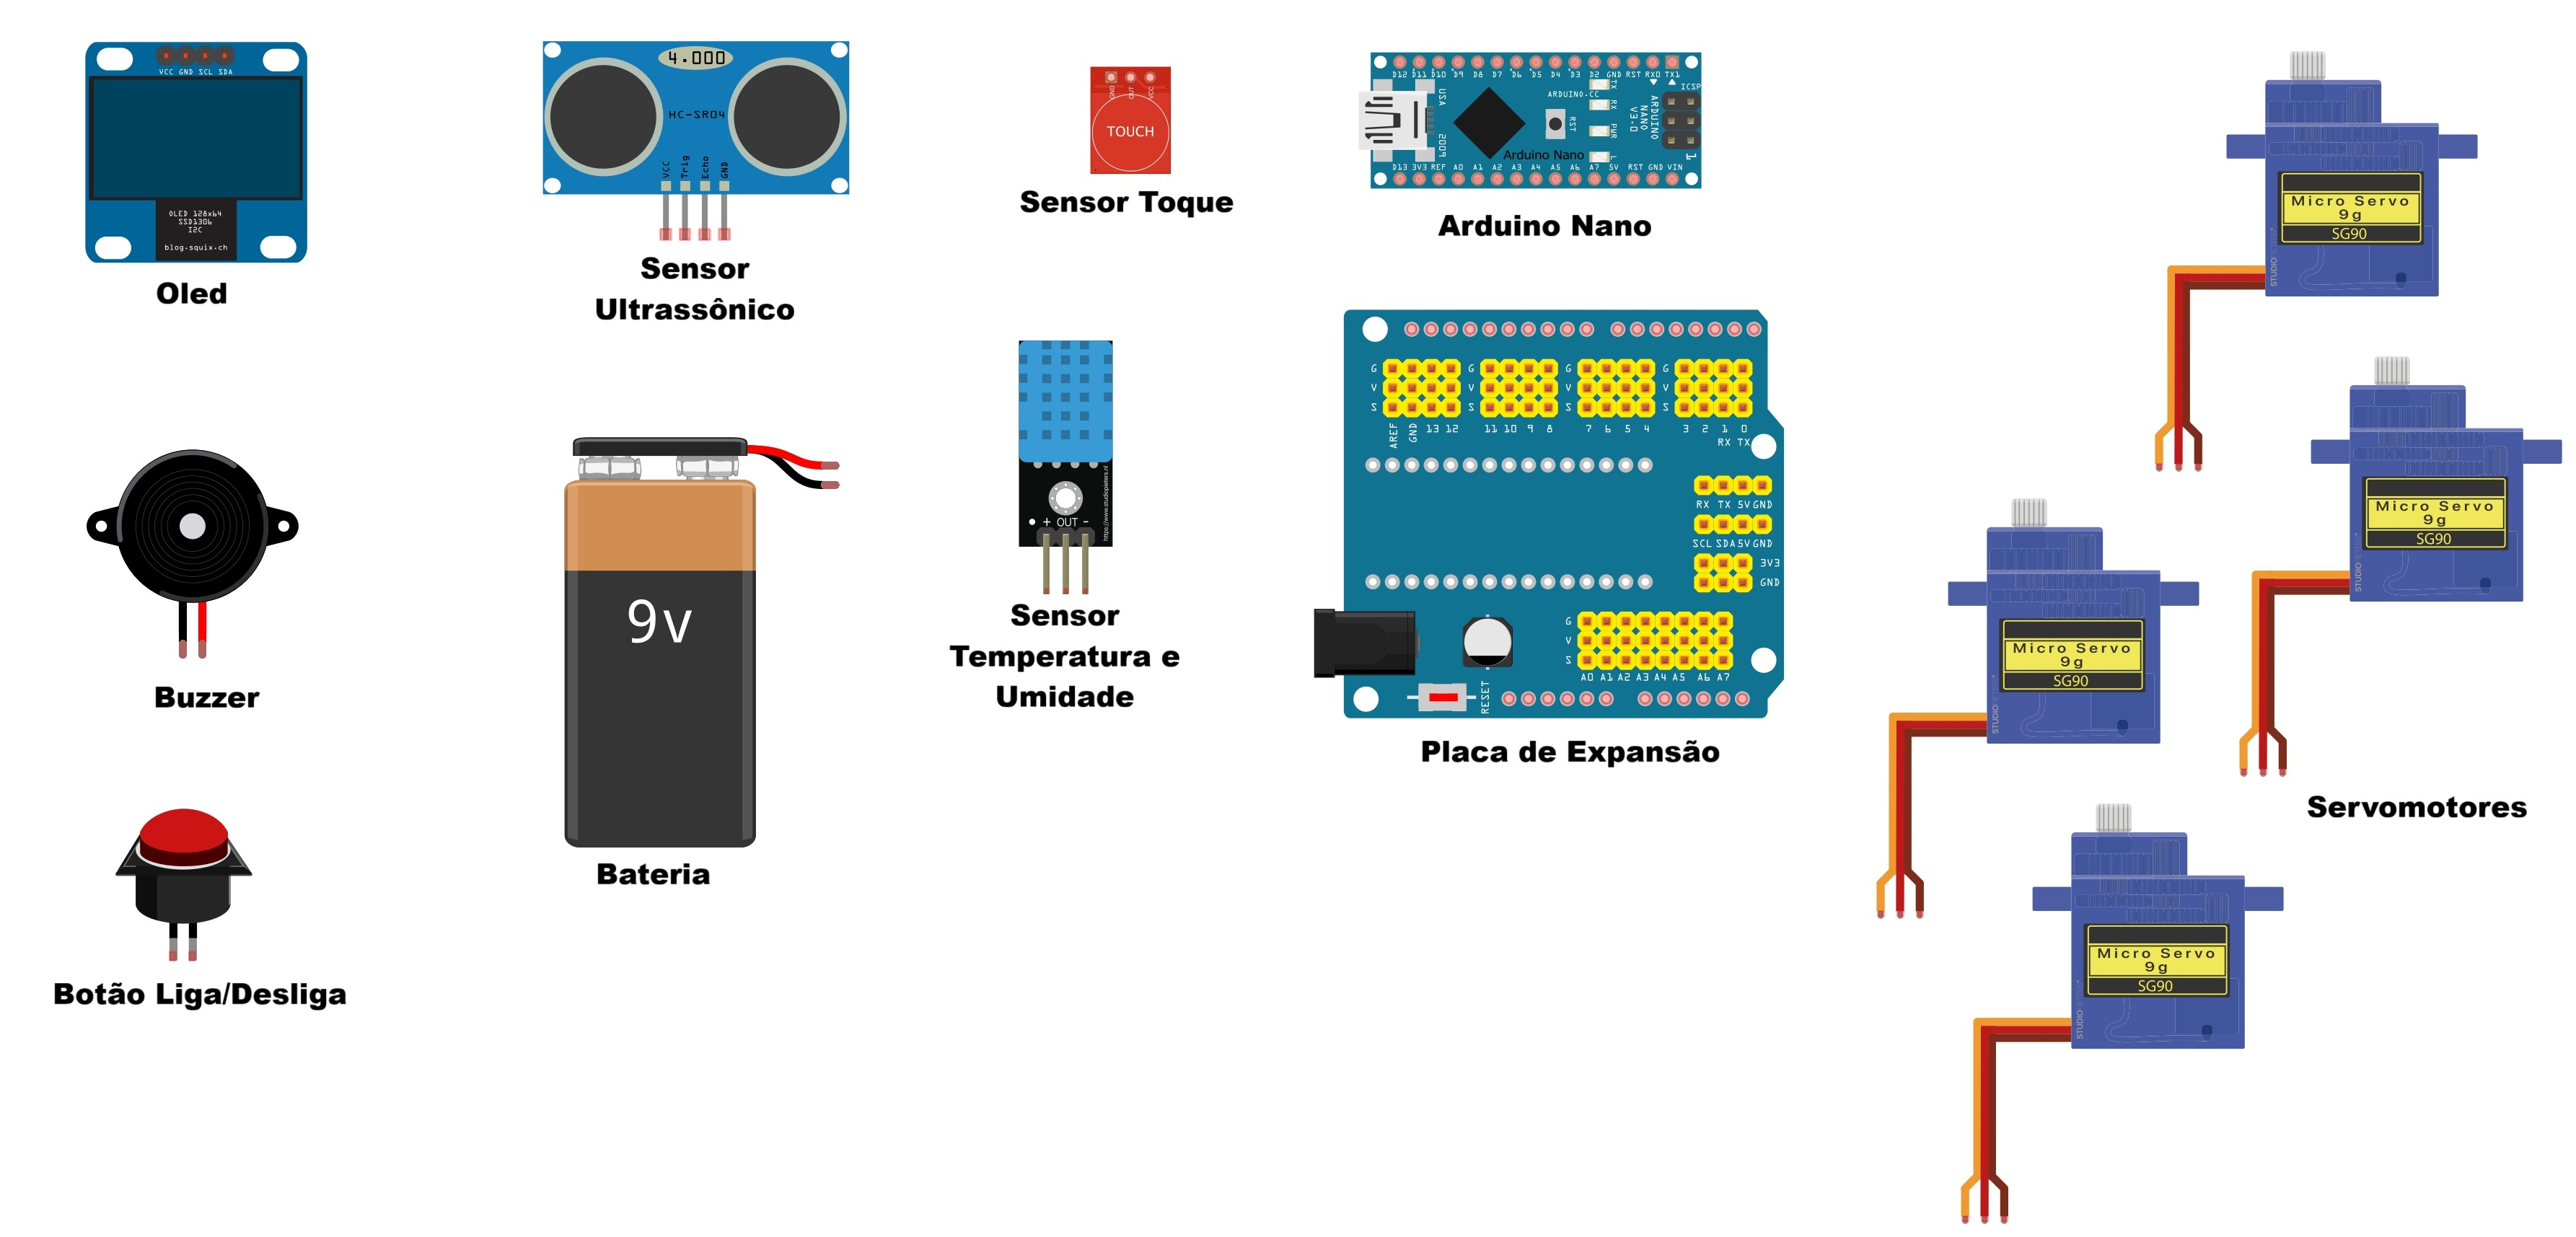
\includegraphics[width=\textwidth]{figures/fig-008.jpg}
		\caption{Componentes eletrônicos.}
		\label{eletronica}
		\source{Autoria Própria.}
	\end{minipage}
\end{figure}


\begin{description}
    \item[Cabeça:] abriga a tela OLED, o sensor toque e o sensor ultrassônico (funcionando como os “olhos” do robô). Essa parte também serve de proteção para a placa Arduino Nano e o módulo de expansão, fixados internamente.
    \item[Corpo:] constitui o compartimento central onde estão alocados os cabos de conexão, buzzer, o sensor de umidade e temperatura, o botão liga/desliga e o suporte para quatro pilhas AA de 1,5V ou uma bateria de 9V, responsáveis pela alimentação do sistema.
    \item[Pernas:] cada perna é articulada por um servomotor, possibilitando o movimento de caminhada e dança. Elas conectam o corpo aos pés, permitindo equilíbrio e coordenação motora.
    \item[Pés:] funcionam como a base de sustentação do robô e alojam dois servomotores adicionais, responsáveis pelo movimento lateral e pelo deslocamento coordenado.
\end{description}

A estrutura do robô foi baseada em modelos da comunidade Otto DIY, o que permitiu o uso de \textit{software} e \textit{hardware} livres. O desenho modular facilita a substituição ou melhoria de partes específicas, o que reforça os princípios da robótica pedagógica livre, permitindo que estudantes explorem aspectos de engenharia, projeto e física mecânica durante o processo de montagem.


\subsection{Desenvolvimento do circuito eletrônico}

A segunda etapa correspondeu à montagem do circuito eletrônico, responsável por integrar todos os sensores, atuadores e módulos de controle do robô. O "coração" do sistema é o Arduino Nano, microcontrolador que gerencia os sinais de entrada e saída de dados. Ele foi acoplado a uma placa de expansão para facilitar as conexões entre os componentes. A Tabela \ref{elementos} é composta pelos elementos do circuito.

\begin{table}[ht!]
		\centering
		\caption{Componentes do protótipo e suas características}
		\label{elementos}
		\begin{tabularx}{\textwidth}{@{}lX@{}}
			\toprule
			Elementos & Características \\
			\midrule
			Servomotores &
			Atuadores responsáveis pelos movimentos dos pés e das pernas; permitem controle de posição angular preciso para movimentos articulados e gestos. \\
			\addlinespace
			Sensor ultrassônico &
			Sensor de distância que utiliza ondas sonoras (ultrassom) para medir intervalos até objetos; empregado na detecção de obstáculos e navegação básica. \\
			\addlinespace
			Sensor de temperatura e umidade &
			Módulo para aquisição de condições ambientais (ex.: DHT11/DHT22); usado para monitorar temperatura e umidade relativa no ambiente. \\
			\addlinespace
			Sensor de toque &
			Dispositivo que detecta contato ou pressão (\textit{touch switch}); usado para ativar respostas interativas ou iniciar rotinas pelo usuário. \\
			\addlinespace
			Tela OLED &
			Display de pequeno porte com alto contraste para exibir textos, ícones ou leituras dos sensores; consome pouca energia e apresenta boa legibilidade. \\
			\addlinespace
			Buzzer &
			Emissor sonoro (ativo ou passivo) responsável por gerar alertas audíveis, sinais de \textit{status} ou \textit{feedback} para interações. \\
			\addlinespace
			Botão liga/desliga e fonte de alimentação &
			Botão para controlar a alimentação do sistema; a fonte de alimentação (ex.: bateria 9\,V) fornece energia portátil ao protótipo, sendo importante prever circuito de proteção. \\
			\addlinespace
			Cabos e fios &
			Condutores elétricos e jumpers usados para realizar conexões de alimentação, sinal e comunicação entre microcontrolador, sensores, atuadores e periféricos. \\
			\addlinespace
			Arduino Nano &
			Placa microcontroladora de código aberto baseada no ATmega328P; oferece entradas/saídas digitais e analógicas, comunicação serial e ambiente de programação acessível (IDE Arduino). \\
			\addlinespace
			Placa de expansão do Arduino Nano &
			Placa auxiliar (\textit{shield}) que facilita a conexão de múltiplos servos, sensores e fontes; normalmente inclui reguladores de tensão, bornes de alimentação e \textit{drivers} para motores. \\
			\bottomrule
		\end{tabularx}
        \source{Autoria Própria.}
\end{table}
	
A modelagem e a montagem das peças em 3D foram realizadas a partir dos arquivos disponibilizados pela comunidade \textit{Otto DIY}, que incentiva o uso e a adaptação de projetos de código aberto voltados à robótica educacional. Cada componente impresso pode ser ajustado e personalizado conforme os objetivos de aprendizagem ou a proposta pedagógica desenvolvida. Esse processo de prototipagem estimula a criatividade, a experimentação e o raciocínio espacial dos estudantes, permitindo compreender de forma prática como a estrutura física do robô influencia seu funcionamento. Ademais, o uso de impressoras 3D e de materiais como o PLA reforça princípios de sustentabilidade e acessibilidade tecnológica, tornando o aprendizado mais envolvente e colaborativo.

A montagem do circuito eletrônico, por sua vez, deve ser guiada pelo conhecimento técnico do professor ou mediador, garantindo o correto posicionamento e a polaridade dos componentes, bem como o controle da corrente elétrica para evitar sobrecargas. Essa etapa é essencial para integrar sensores e atuadores em um sistema funcional, no qual o robô é capaz de perceber o ambiente, emitir sinais sonoros e executar movimentos de forma coordenada. O trabalho com circuitos também desenvolve a compreensão dos alunos sobre princípios de eletrônica e programação embarcada, aproximando teoria e prática no contexto educacional. A Figura~\ref{circuito} apresenta o diagrama do circuito eletrônico do robô, com todas as conexões visíveis. A partir desse esquema, é possível reproduzir o mesmo modelo ou adaptar novas configurações conforme as demandas de cada projeto pedagógico.

\begin{figure}[ht!]
	\centering
	\begin{minipage}{.75\textwidth}		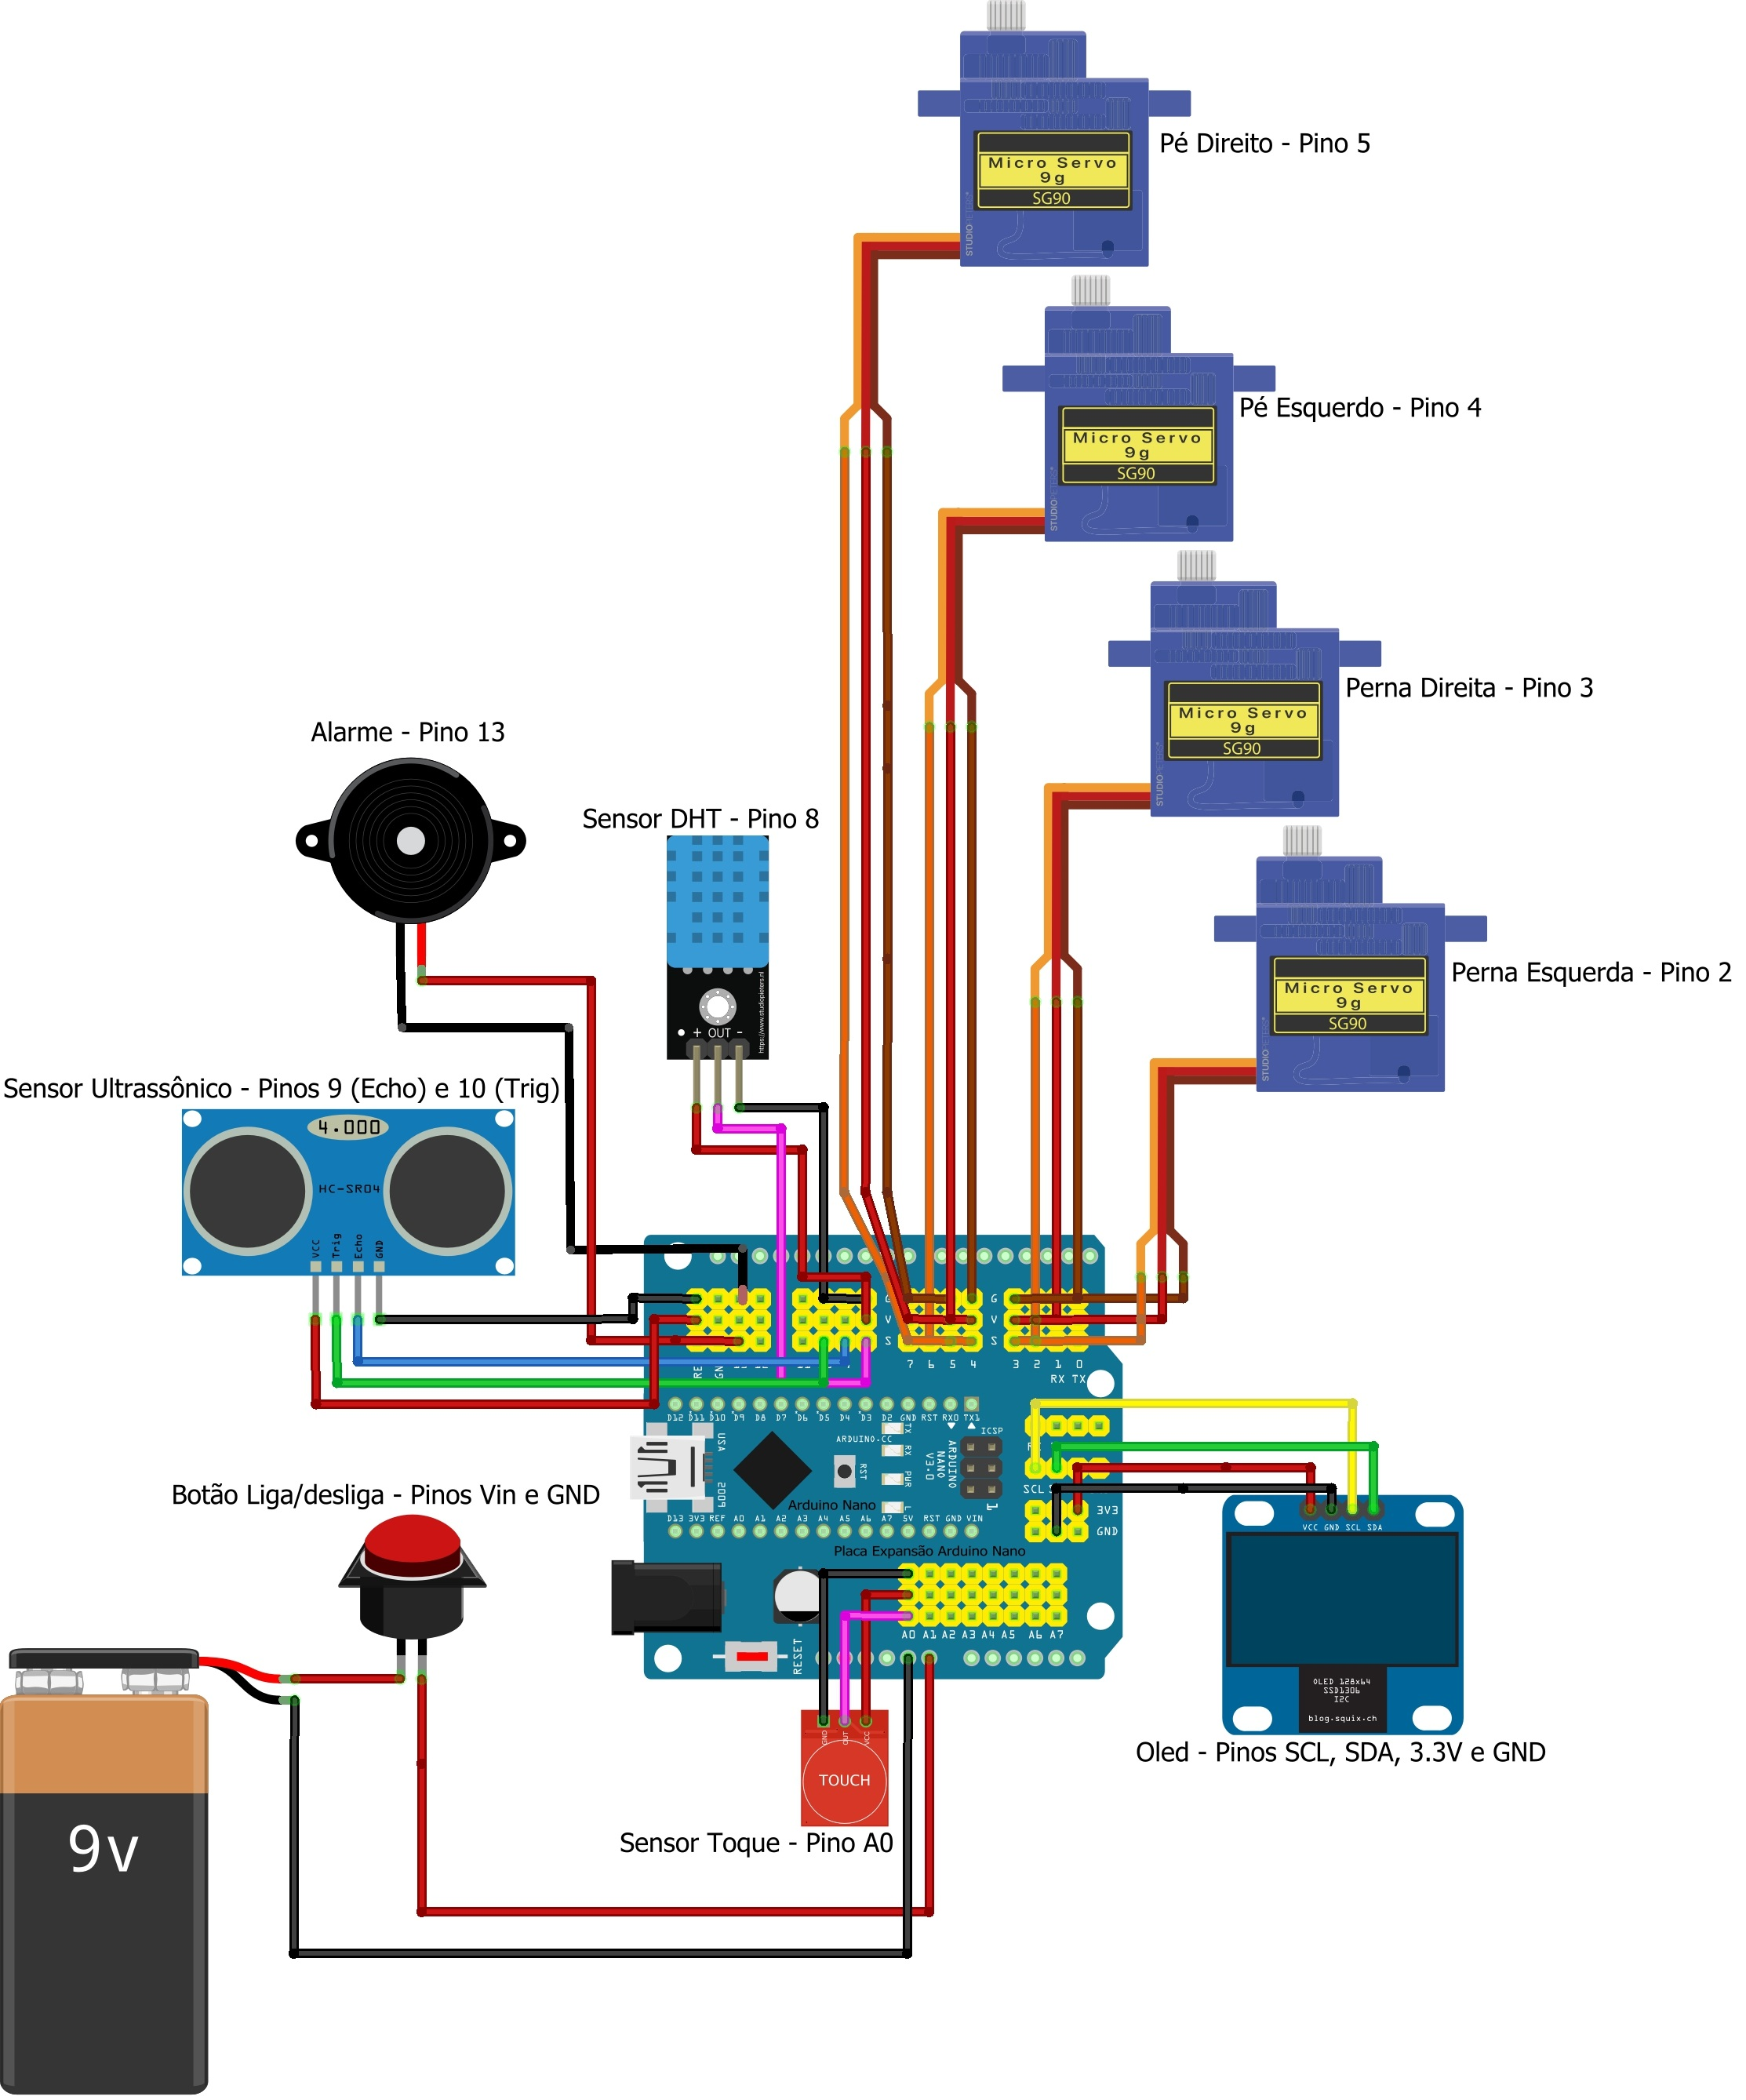
\includegraphics[width=\textwidth]{figures/fig-009.jpg}
		\caption{Circuito eletrônico do robô.}
		\label{circuito}
		\source{Autoria Própria.}
	\end{minipage}
\end{figure}

Nota-se de forma clara a organização do circuito eletrônico e a interconexão entre os principais componentes do robô. A partir dessa representação visual, é possível compreender como cada elemento contribui para o funcionamento do sistema integrado, evidenciando a importância do planejamento e da execução cuidadosa de cada etapa. Conclui-se que o processo de montagem, desde a impressão das peças em 3D até a configuração dos circuitos, não apenas resulta em um produto funcional, mas também constitui uma experiência educativa completa, que desperta o interesse dos alunos pela ciência, tecnologia e engenharia. Assim, a robótica pedagógica se consolida como uma ferramenta transformadora no ensino, promovendo autonomia, criatividade e aprendizagem significativa.

\subsection{Código-fonte aberto}

A etapa de programação consistiu no desenvolvimento e personalização do código-fonte responsável por controlar o robô. O \textit{software} foi criado na plataforma Arduino IDE, utilizando linguagens de programação baseadas em C/C++ e bibliotecas específicas, como "Servo.h" (controle de servomotores), "Adafruit\_SSD1306.h" (exibição na tela OLED), "DHT.h" (leitura de temperatura e umidade) e "NewPing.h" (leitura de distância com o sensor ultrassônico).

O código foi estruturado em módulos funcionais, permitindo a execução de diferentes tarefas conforme o tipo de atividade planejada. Cada módulo corresponde a uma tarefa pedagógica, programadas para relacionar medições físicas ou matemáticas com movimentos e respostas do robô, por exemplo:

\begin{itemize}
	\item exibir dados de temperatura e umidade na tela OLED;
	\item acionar movimentos de acordo com a distância detectada;
	\item representar funções matemáticas por meio de padrões de movimento.
\end{itemize}

Durante o desenvolvimento, os estudantes terão contato direto com a lógica de programação, realizando as modificações no código e observando os resultados práticos, o que favorece o aprendizado de pensamento computacional e o fortalecimento do raciocínio lógico-matemático.

Os trechos de código apresentados da \Cref{lista1} até a \cref{lista4} foram desenvolvidos na linguagem \textit{C++} utilizando a plataforma Arduino, com o objetivo de programar e controlar o robô educacional RoboJoy. As listagens contemplam a estrutura completa do sistema embarcado, abrangendo desde a inicialização de bibliotecas e definição de variáveis até as rotinas de movimentação, sensoriamento e exibição de dados no display OLED. Cada bloco de código foi comentado linha a linha para facilitar a compreensão das funções implementadas, destacando o papel de cada componente: servomotores, sensores, buzzer e tela na execução das tarefas do robô. Essa abordagem favorece a análise didática do funcionamento do sistema e permite que os estudantes repliquem ou adaptem o projeto em diferentes contextos de ensino e pesquisa.

\begin{lstlisting}[language=C, label=lista1, caption={Definição da biblioteca e dos pinos dos sensores.},postbreak=\mbox{$\hookrightarrow$\space}]
// Elaborado por Juliana Almansa Malagoli
// ==== Bibliotecas ====
#include <Servo.h>                 // Controle dos servomotores
#include <Adafruit_GFX.h>          // Usada com o display OLED
#include <Adafruit_SSD1306.h>      // Para o display OLED SSD1306
#include "DHT.h"                   // Temperatura e umidade (sensor DHT11)
#include <PlayRtttl.hpp>           // Reproduzir melodias (buzzer)
#include <NewPing.h>               // Distância com o sensor ultrassônico.

// ==== OLED ====
#define SCREEN_WIDTH 128           // Largura do display OLED em pixels
#define SCREEN_HEIGHT 64           // Altura do display OLED em pixels
#define OLED_RESET -1              // Pino reset OLED (-1 indica sem uso)
Adafruit_SSD1306 display(SCREEN_WIDTH, SCREEN_HEIGHT, & Wire, OLED_RESET); // Cria o objeto do display com os parâmetros definidos

// ==== Sensores ====
#define DHTPIN 8                   // Pino digital 8 para o sensor DHT11
DHT dht_1(DHTPIN, DHT11);          // Cria um objeto DHT no pino 8 
#define TRIG 10                    // Pino 10 do trigger do ultrassônico
#define ECHO 9                     // Pino 9 para o echo do ultrassônico
#define TOUCH A0                   // Pino analógico A0, sensor de toque
#define BUZZER 13                  // Pino digital 13 para o buzzer (som)

// ==== Servos das pernas ====
Servo LeftLeg;                     // Cria o objeto para a perna esquerda
Servo RightLeg;                    // Cria o objeto para a perna direita
Servo LeftFoot;                    // Cria o objeto para o pé esquerdo
Servo RightFoot;                   // Cria o objeto para o pé direito
\end{lstlisting}

\begin{lstlisting}[language=C, label=lista2, caption={Controles das configurações, funções de movimento e etapas.},postbreak=\mbox{$\hookrightarrow$\space}]
// Elaborado por Juliana Almansa Malagoli
// ===== Configurações =====
int repetitions = 2;      // Quantas vezes cada movimento será repetido
int stepDelay = 60;       // Tempo de atraso entre incrementos de movimento
int intervalBetweenMoves = 500; // Intervalo de espera entre movimentos

// ===== Função para movimento suave =====
void smoothMove(Servo & servo, int fromAngle, int toAngle, int stepDelay) {
// Se o ângulo inicial for < que o final
	if(fromAngle < toAngle) {  
		// Incrementa o ângulo gradualmente
		for(int a = fromAngle; a < = toAngle; a++) { 
			// Move o servo para o ângulo atual
			servo.write(a);        
			// Pequeno atraso para suavizar o movimento
			delay(stepDelay/10);   
		}
	} else { // Caso o ângulo inicial seja > que o final
		// Decrementa o ângulo gradualmente
		for(int a = fromAngle; a > = toAngle; a--) { 
			// Move o servo para o ângulo atual
			servo.write(a);        
			// Pequeno atraso para suavizar o movimento
			delay(stepDelay/10);   
		}}}

// ==== Controle de etapas ====
int etapa = 0; // Variável que armazena a etapa atual do movimento

// ==== Função ultrassônico ====
long ultrasound_distance_simple() {
	digitalWrite(TRIG, LOW);        // Pino TRIG comece em nível baixo
	delayMicroseconds(2);           // Espera 2 microssegundos
	digitalWrite(TRIG, HIGH);   // Pulso de 10 microssegundos no TRIG
	delayMicroseconds(10);
	digitalWrite(TRIG, LOW);        // Retorna o TRIG ao nível baixo
	long duration = pulseIn(ECHO, HIGH); // Mede o tempo no pino ECHO
	long distance = duration * 0.034 / 2; // Converte o T em Dist (cm)
	if(distance == 0) 
	distance = 200;  // Proteção contra leitura inválida
	return distance;                      // Retorna a distância medida
}

\end{lstlisting}

Com o objetivo de complementar a análise e possibilitar uma melhor compreensão dos movimentos de dança executados pelo RoboJoy, foi disponibilizado um arquivo no formato .cpp, contendo exclusivamente as rotinas responsáveis pelas sequências coreográficas do robô. Essa disponibilização visa evitar o excesso de listagens de código no corpo do trabalho, mantendo a fluidez textual e a clareza da apresentação. Para facilitar o acesso, foi inserido um código QR (Figura \ref{fig_danca}) que direciona o leitor ao arquivo, permitindo a consulta e a reprodução dos movimentos programados.

\begin{figure}[ht!]
	\centering
	\begin{minipage}{.3\textwidth}		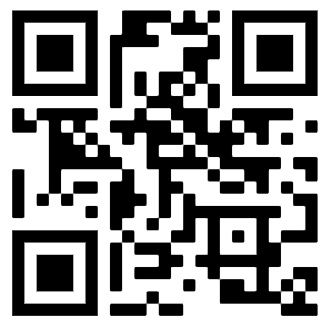
\includegraphics[width=\textwidth]{figures/fig-010.jpg}
		\caption{Arquivo .cpp com a coreografia do RoboJoy.}
		\label{fig_danca}
		\source{Autoria Própria.}
	\end{minipage}
\end{figure}


\begin{lstlisting}[language=C, label=lista3, caption={Função para mostrar tela inicial e configurações.},postbreak=\mbox{$\hookrightarrow$\space}]
// Elaborado por Juliana Almansa Malagoli
// ==== Função para mostrar tela inicial ====
void mostrarTelaInicial() {   // Exibe a tela inicial no display OLED
	display.clearDisplay();   // Limpa o conteúdo anterior do display
	display.setTextSize(2.2);   // Define o tamanho da fonte
	display.setTextColor(WHITE);   // Define a cor do texto como branca
	display.setCursor(20,22);   // Posiciona o cursor na tela
	display.println("RoboJoy");   // Mostra o nome "RoboJoy"
	// Desenha uma borda arredondada
	display.drawRoundRect(1, 1, 126, 62, 10, WHITE); 
	display.display();   // Atualiza o display para mostrar tudo
}

// ==== Configurações ====
void setup() {
	// Servos
	LeftLeg.attach(2);   // Conecta o servo da perna esquerda ao pino 2
	RightLeg.attach(3);   // Conecta o servo da perna direita ao pino 3
	LeftFoot.attach(4);   // Conecta o servo do pé esquerdo ao pino 4
	RightFoot.attach(5);   // Conecta o servo do pé direito ao pino 5
	
	// Sensores
	pinMode(TRIG, OUTPUT);   // Define o pino TRIG como saída
	pinMode(ECHO, INPUT);   // Define o pino ECHO como entrada
	// Define o pino do sensor de toque como entrada
	pinMode(TOUCH, INPUT);   
	dht_1.begin();   // Inicializa o sensor de temperatura e umidade
	
	// OLED
	// Inicializa o display OLED no endereço 0x3C
	display.begin(SSD1306_SWITCHCAPVCC, 0x3C);   
	display.clearDisplay();   // Limpa a tela
	display.display();   // Atualiza o display
	
	// Tela inicial
	mostrarTelaInicial();   // Mostra a tela de boas-vindas
	// Emite som no buzzer: 1000 Hz por 200 ms
	tone(BUZZER, 1000, 200);   
	delay(250);   // Pequena pausa entre sons
	noTone(BUZZER);   // Interrompe o som
}

// ==== Repetição ====
void loop() {
	// Se o sensor de toque for ativado
	if(digitalRead(TOUCH) == HIGH){   
		delay(200);   // Pequeno atraso (debounce)
		executarEtapa();   // Executa uma etapa de movimento
	}
}
\end{lstlisting}

\begin{lstlisting}[language=C, label=lista4, caption={Execução das etapas.},postbreak=\mbox{$\hookrightarrow$\space}]
	// Elaborado por Juliana Almansa Malagoli
	// ==== Executar etapa ====
	void executarEtapa() {
		display.clearDisplay();   // Limpa o display OLED
		display.setTextSize(2);   // Define o tamanho da fonte
		// Define a cor do texto como branca
		display.setTextColor(WHITE);   
		// Etapa 1: Leitura de temperatura e umidade
		if(etapa == 0){   
			display.clearDisplay();               
			display.setCursor(10,10);             
			// Exibe temperatura ajustada
			display.println(round(dht_1.readTemperature()-2)); 
			display.setCursor(35,10);
			// Indica unidade de temperatura             
			display.println(".C Temp");           
			display.setCursor(10,48);             
			// Exibe umidade ajustada
			display.println(round(dht_1.readHumidity()+2));    
			display.setCursor(38,48);             
			// Indica unidade de umidade
			display.println("% Umid");            
			// Atualiza o display com os valores 
			display.display();                    
			
			// Faz o robô piscar os pés duas vezes
			for(int i=0;i<2;i++){
				liftBothFeet(); 
				lowerBothFeet(); 
			}
			
			// Som breve do buzzer
			tone(BUZZER,1500,200); delay(250); noTone(BUZZER); 
			etapa = 1;   // Passa para a próxima etapa
		} 
		
		// Etapa 2: Detecção de distância
		else if(etapa == 1){                    
			display.clearDisplay();
			display.setCursor(20,28);
			// Mensagem de movimento
			display.println("Anda..");            
			display.display();
			moveForward(); 
			
			// Move o robô para frente
			delay(intervalBetweenMoves); 
			
			// Se distância menor que 15 cm, recua
			if (ultrasound_distance_simple() < 15){
				moveBackward(); 
				delay(intervalBetweenMoves);
			}
			// Sinal sonoro
			tone(BUZZER,1500,200); delay(250); noTone(BUZZER); 
			etapa = 2;   // Passa para a etapa seguinte
		}
		
		// Etapa 3: Dança
		else if(etapa == 2){                    
			display.clearDisplay();
			display.setCursor(20,28);
			// Mensagem "Dance.."
			display.println("Dance..");           
			display.display();
			// Movimentos iniciais
			liftBothFeet(); lowerBothFeet();      
			// Pequenas vibrações
			jitter(); delay(intervalBetweenMoves); 
			// Movimento de balanço
			swing(); delay(intervalBetweenMoves);  
			// Sacode perna direita
			shakeRightLeg(); delay(intervalBetweenMoves); 
			// Sacode perna esquerda
			shakeLeftLeg(); delay(intervalBetweenMoves);  
			// Movimento de sobe e desce
			upDown(); delay(intervalBetweenMoves);        
			// Finaliza com som
			tone(BUZZER,1500,200); delay(250); noTone(BUZZER); 
			mostrarTelaInicial();   // Retorna à tela inicial
			etapa = 0;   // Reinicia o ciclo
		}
	}
	
\end{lstlisting}

A implementação completa do código demonstra a integração entre os módulos de \textit{hardware} e \textit{software} do RoboJoy, evidenciando a lógica de controle e a resposta interativa do robô frente aos estímulos dos sensores. A combinação entre os servomotores, o sensor ultrassônico, o sensor de toque, o sensor de temperatura e umidade e o \textit{buzzer}, coordenados pelo microcontrolador Arduino, permite a execução autônoma de movimentos e ações programadas. Essa estrutura modular possibilita a expansão do sistema para novas funcionalidades e promove um ambiente de aprendizado ativo, em que os estudantes podem compreender conceitos fundamentais de eletrônica, programação e automação de maneira prática e envolvente.


\section{Resultados e discussões}\label{sec-resultados}

Esta seção apresenta propostas de atividades pedagógicas que poderão ser desenvolvidas com estudantes utilizando o robô Otto DIY. O protótipo inicial foi construído pela professora com o objetivo de servir como modelo para as atividades didáticas. Os estudantes poderão participar da construção de novos robôs utilizando componentes acessíveis e materiais de baixo custo, favorecendo o aprendizado sobre montagem, eletrônica e programação.

As atividades serão desenvolvidas em um ambiente colaborativo, no qual os estudantes poderão assumir papéis ativos na experimentação e exploração dos recursos do robô. A proposta busca integrar teoria e prática por meio de atividades relacionadas aos conteúdos de Termodinâmica, Ondas Sonoras, Cinemática, Estatística, Trigonometria e Funções Lineares, incentivando a investigação e a aprendizagem por experimentação.

Durante as atividades, os estudantes poderão realizar medições de temperatura, umidade e distância utilizando os sensores do RoboJoy, registrando os dados para posterior análise estatística. Além disso, poderão explorar
os servomotores em atividades que abordam movimento e trigonometria, compreendendo relações entre ângulos e deslocamento.

\subsection{Desenvolvimento e funcionamento do RoboJoy}

O RoboJoy, desenvolvido pela autora, é uma versão aprimorada do modelo Otto DIY, construído com peças impressas em 3D (material PLA) e equipado com Arduino Nano, sensor ultrassônico, sensor de umidade e temperatura, sensor de toque, display OLED, buzzer, quatro servomotores, fios e bateria. A proposta central desta atividade é apresentar o funcionamento integrado do robô, articulando conceitos de física, matemática e programação em um contexto de aprendizagem ativa e interdisciplinar.

O código implementado no ambiente Arduino IDE foi projetado com uma lógica modular, integrando sensores e atuadores em três etapas distintas de execução, controladas pelo toque do usuário. O display OLED exibe os dados de leitura e mensagens de status, enquanto o buzzer fornece retorno sonoro durante as transições de cada fase. A função `smoothMove()` garante movimentos suaves, aprimorando o comportamento cinemático do robô.

As etapas de funcionamento do robô RoboJoy podem ser observadas nas Figuras \ref{fig_robojoy} a \ref{fig_dance}, que ilustram desde sua estrutura física até as diferentes execuções programadas no código. A Figura \ref{fig_robojoy} apresenta o modelo completo desenvolvido pela autora, evidenciando a integração entre os componentes eletrônicos e a estrutura impressa em 3D. Na Figura \ref{fig_temp}, observa-se as leituras de temperatura e umidade, realizadas pelo sensor DTH11, com a exibição dos dados em tempo real no display OLED. 

Já a Figura \ref{fig_ande} mostra o Robojoy andando para frente sem obstáculo e para trás depois de ter um objeto a sua frente, movimentos realizados através do sensor ultrassônico. Por fim, a Figura \ref{fig_dance} demonstra a execução da rotina de dança, na qual os servomotores atuam de forma sincronizada, representando a aplicação prática dos conceitos de movimento e programação. Adicionalmente, a Tabela~\ref{tab:funcoes_robojoy} apresenta um resumo das principais funções do programa, descrevendo sua relação com os conceitos de física e matemática e os objetivos pedagógicos associados.


\begin{figure}[ht!] 
\centering
\begin{minipage}{0.75\textwidth}
	\begin{minipage}[t]{0.45\textwidth}
		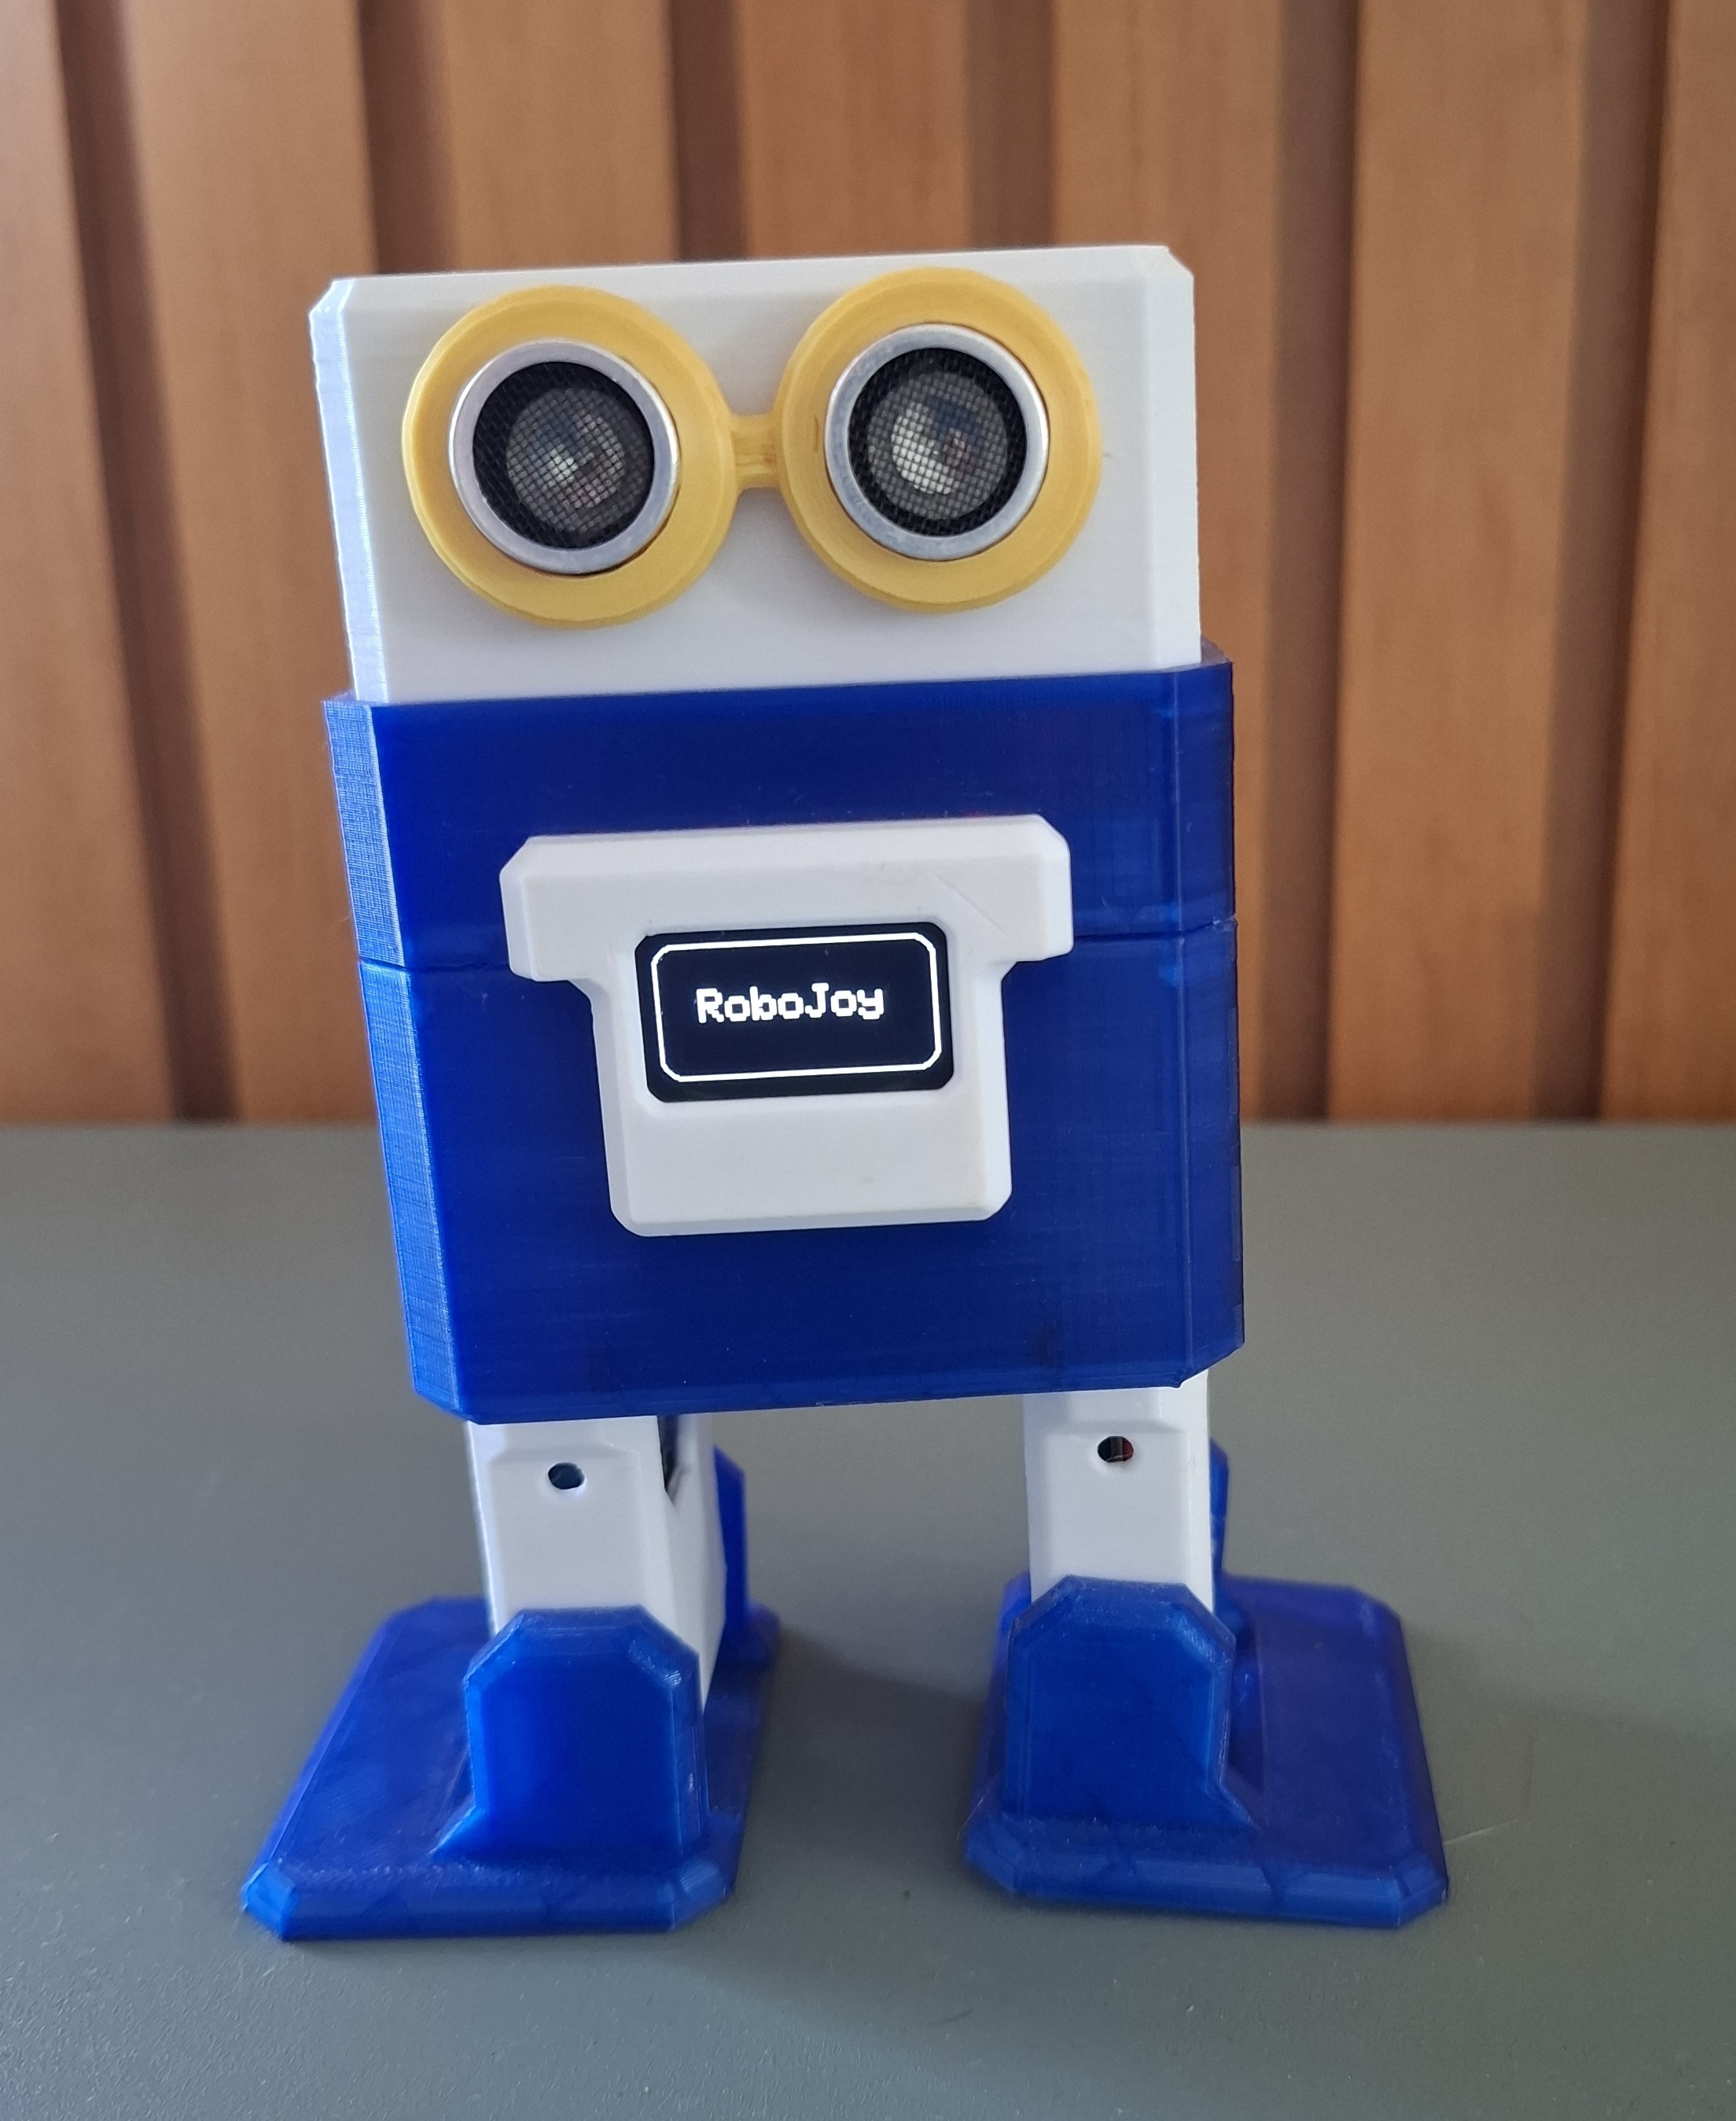
\includegraphics[width=\linewidth]{figures/fig-011a.jpg}
		\subcaption{Frente do robô.}
	\end{minipage}
	\hfill
	\begin{minipage}[t]{0.43\textwidth}
		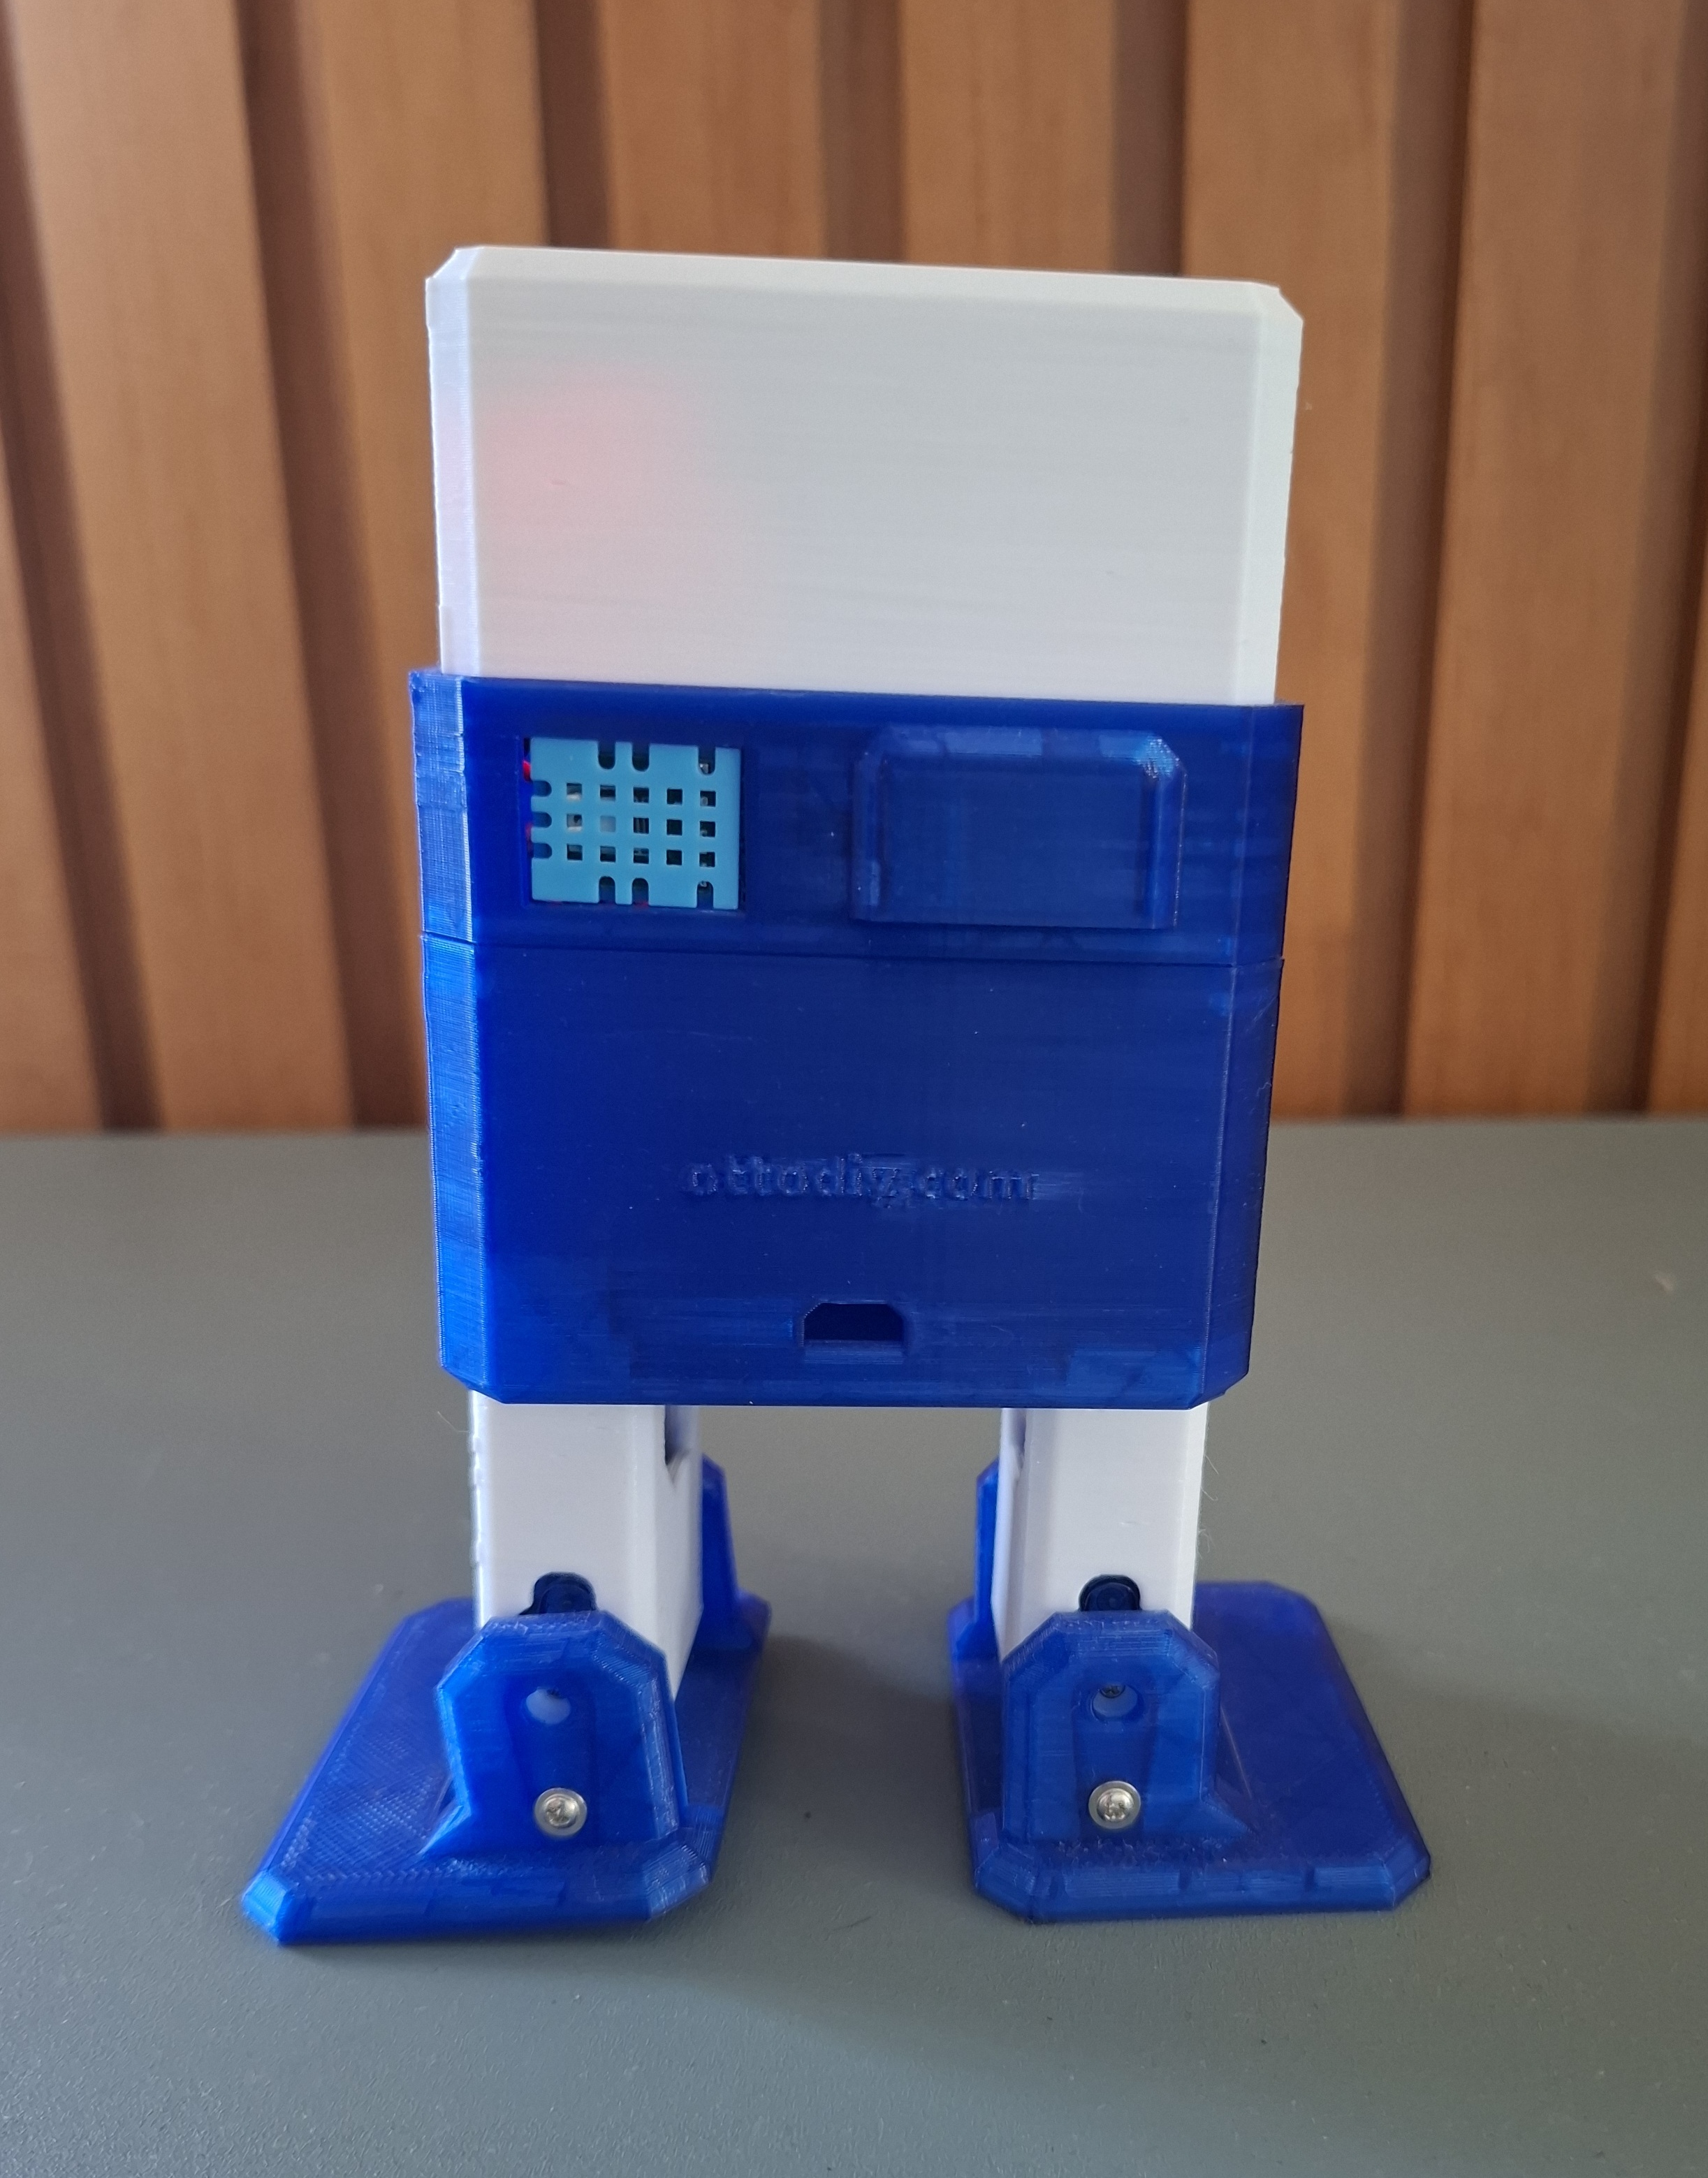
\includegraphics[width=\linewidth]{figures/fig-011b.jpg}
		\subcaption{Traseira do robô.}
	\end{minipage}
	\caption{Estrutura completa montada do Robô.}
	\label{fig_robojoy}
	\source{Autoria Própria.}
\end{minipage}
\end{figure}


\begin{figure}[ht!]
	\centering
	\begin{minipage}{.32\textwidth}
    
\includegraphics[width=\textwidth]{figures/fig-012.jpg}
		\caption{Medição de temperatura e umidade com exibição no OLED.}
		\label{fig_temp}
		\source{Autoria Própria.}
	\end{minipage}
\end{figure}


\begin{figure}[ht!]
\begin{minipage}{0.75\textwidth}
	\begin{minipage}[t]{0.45\textwidth}
		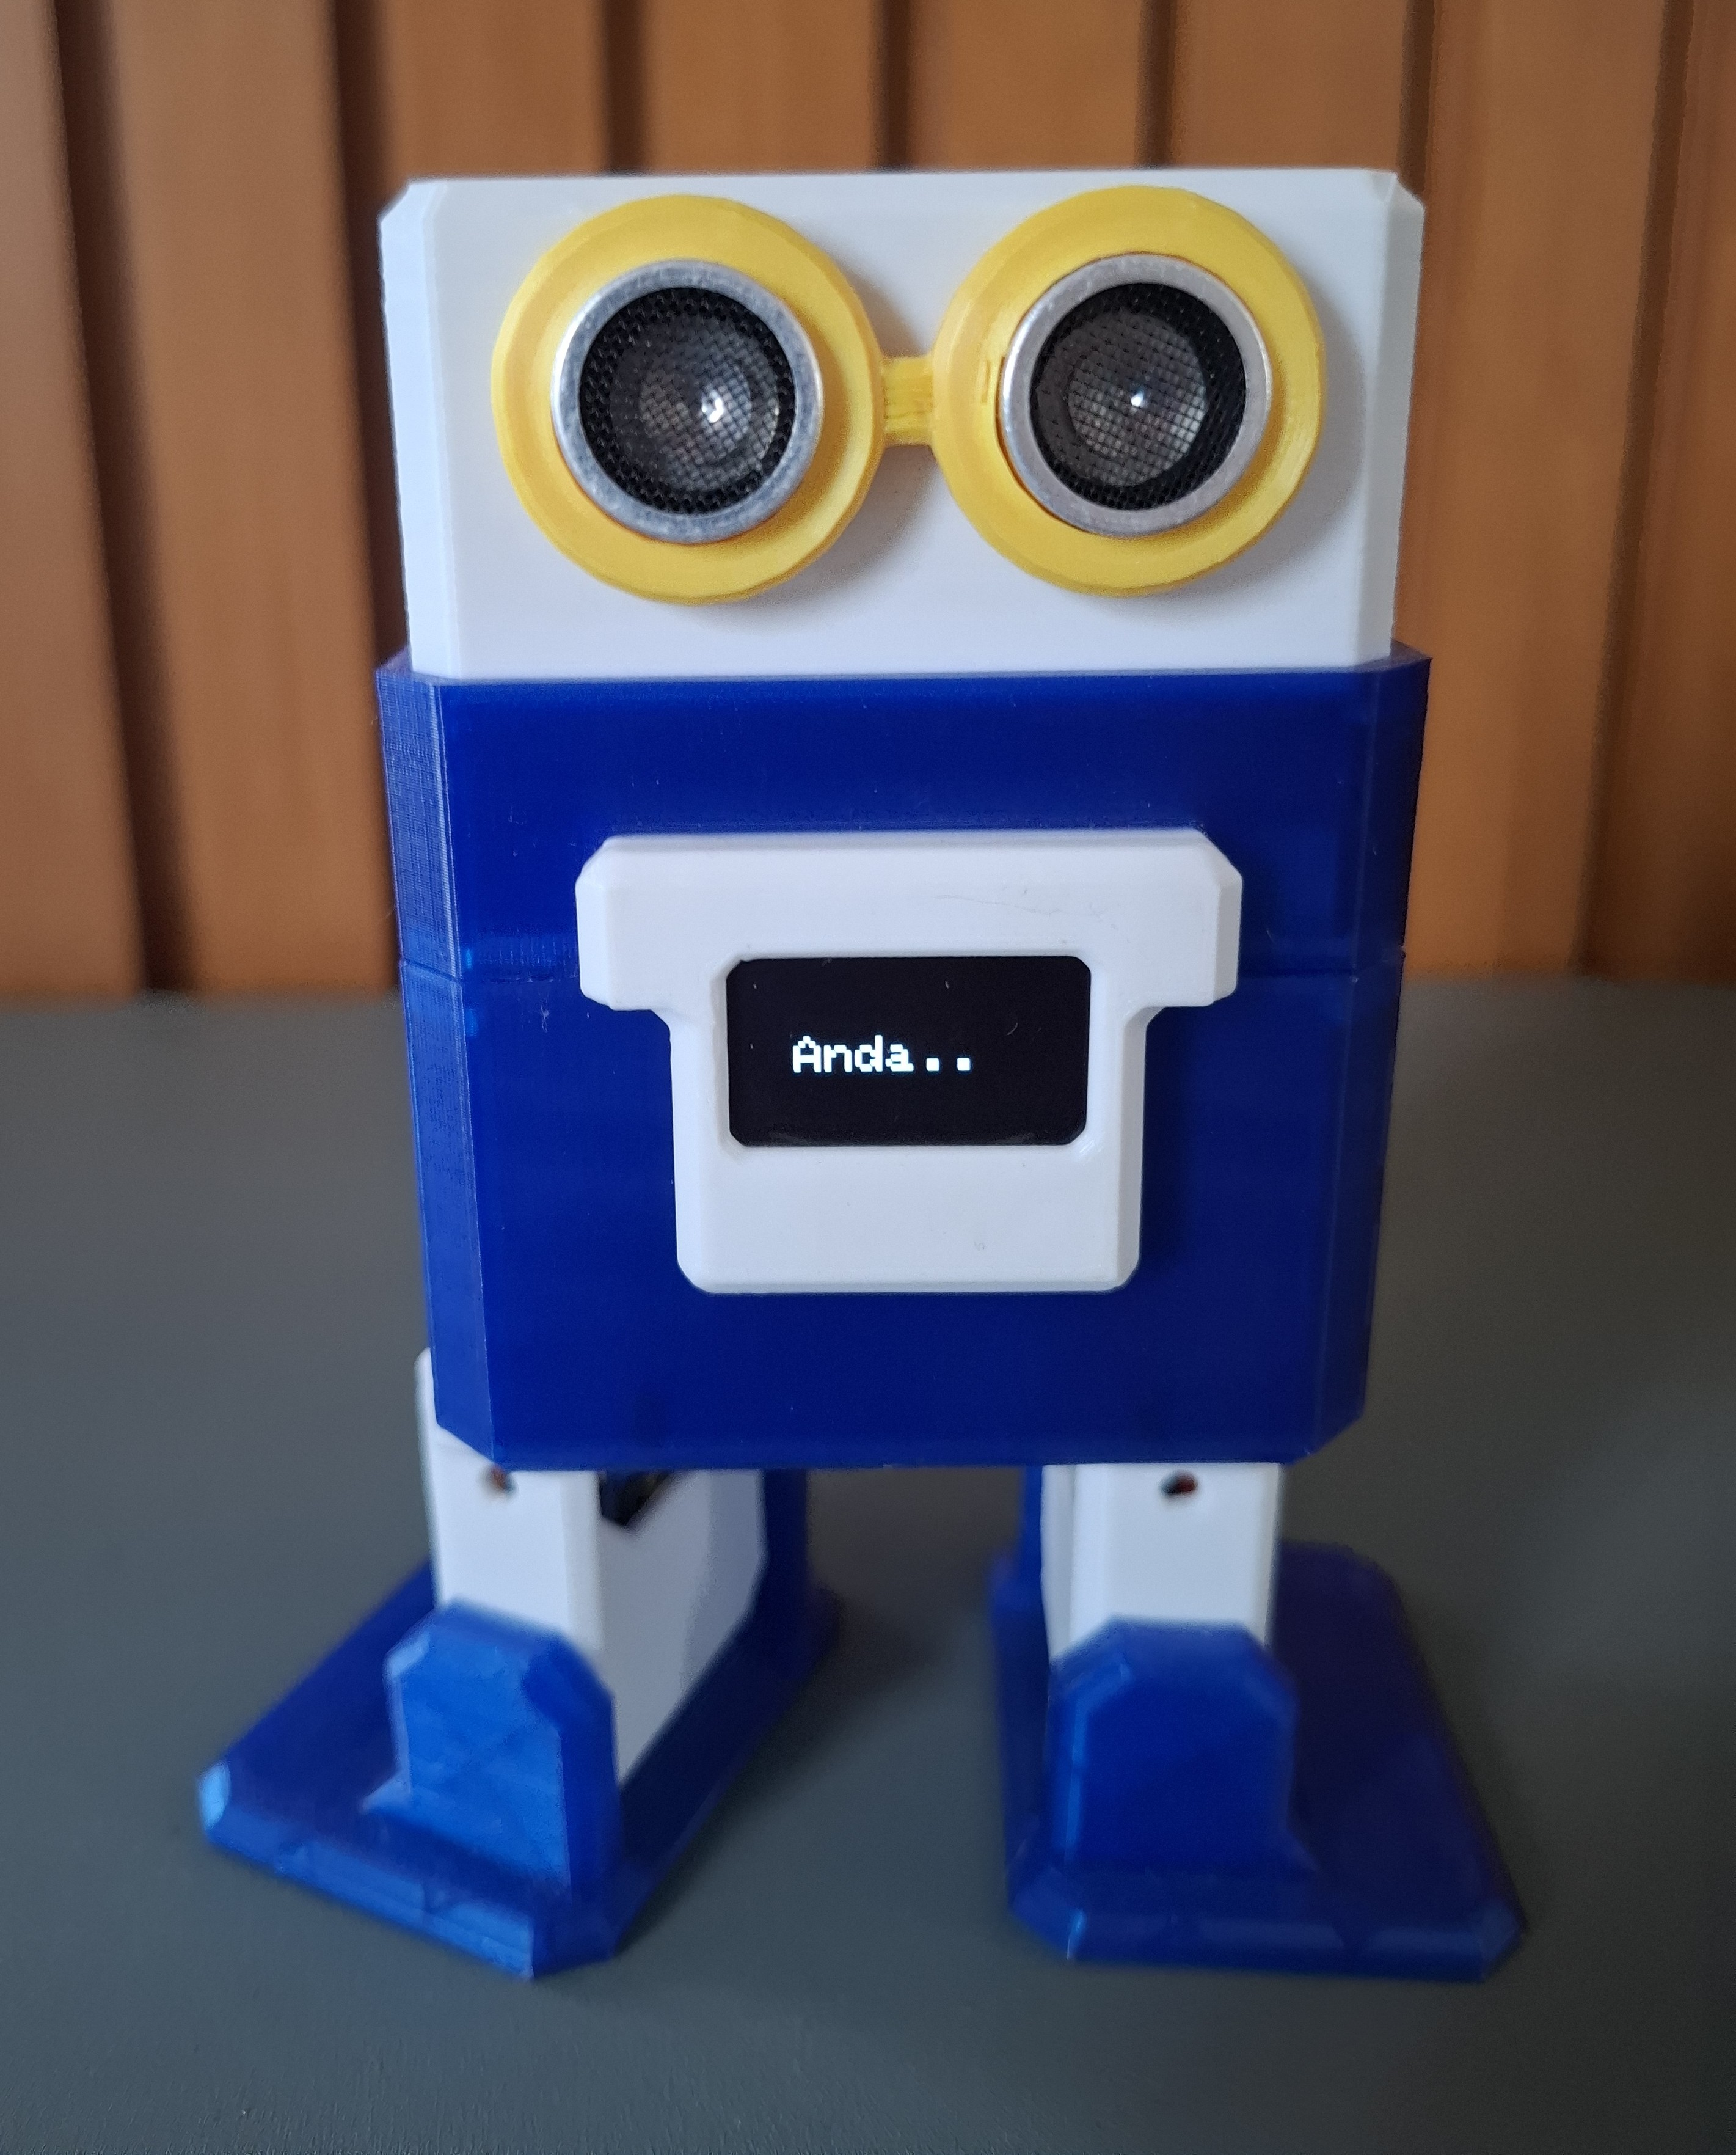
\includegraphics[width=\linewidth]{figures/fig-013a.jpg}
		\subcaption{RoboJoy andando para frente sem obstáculo.}
	\end{minipage}
	\hfill
	\begin{minipage}[t]{0.41\textwidth}
		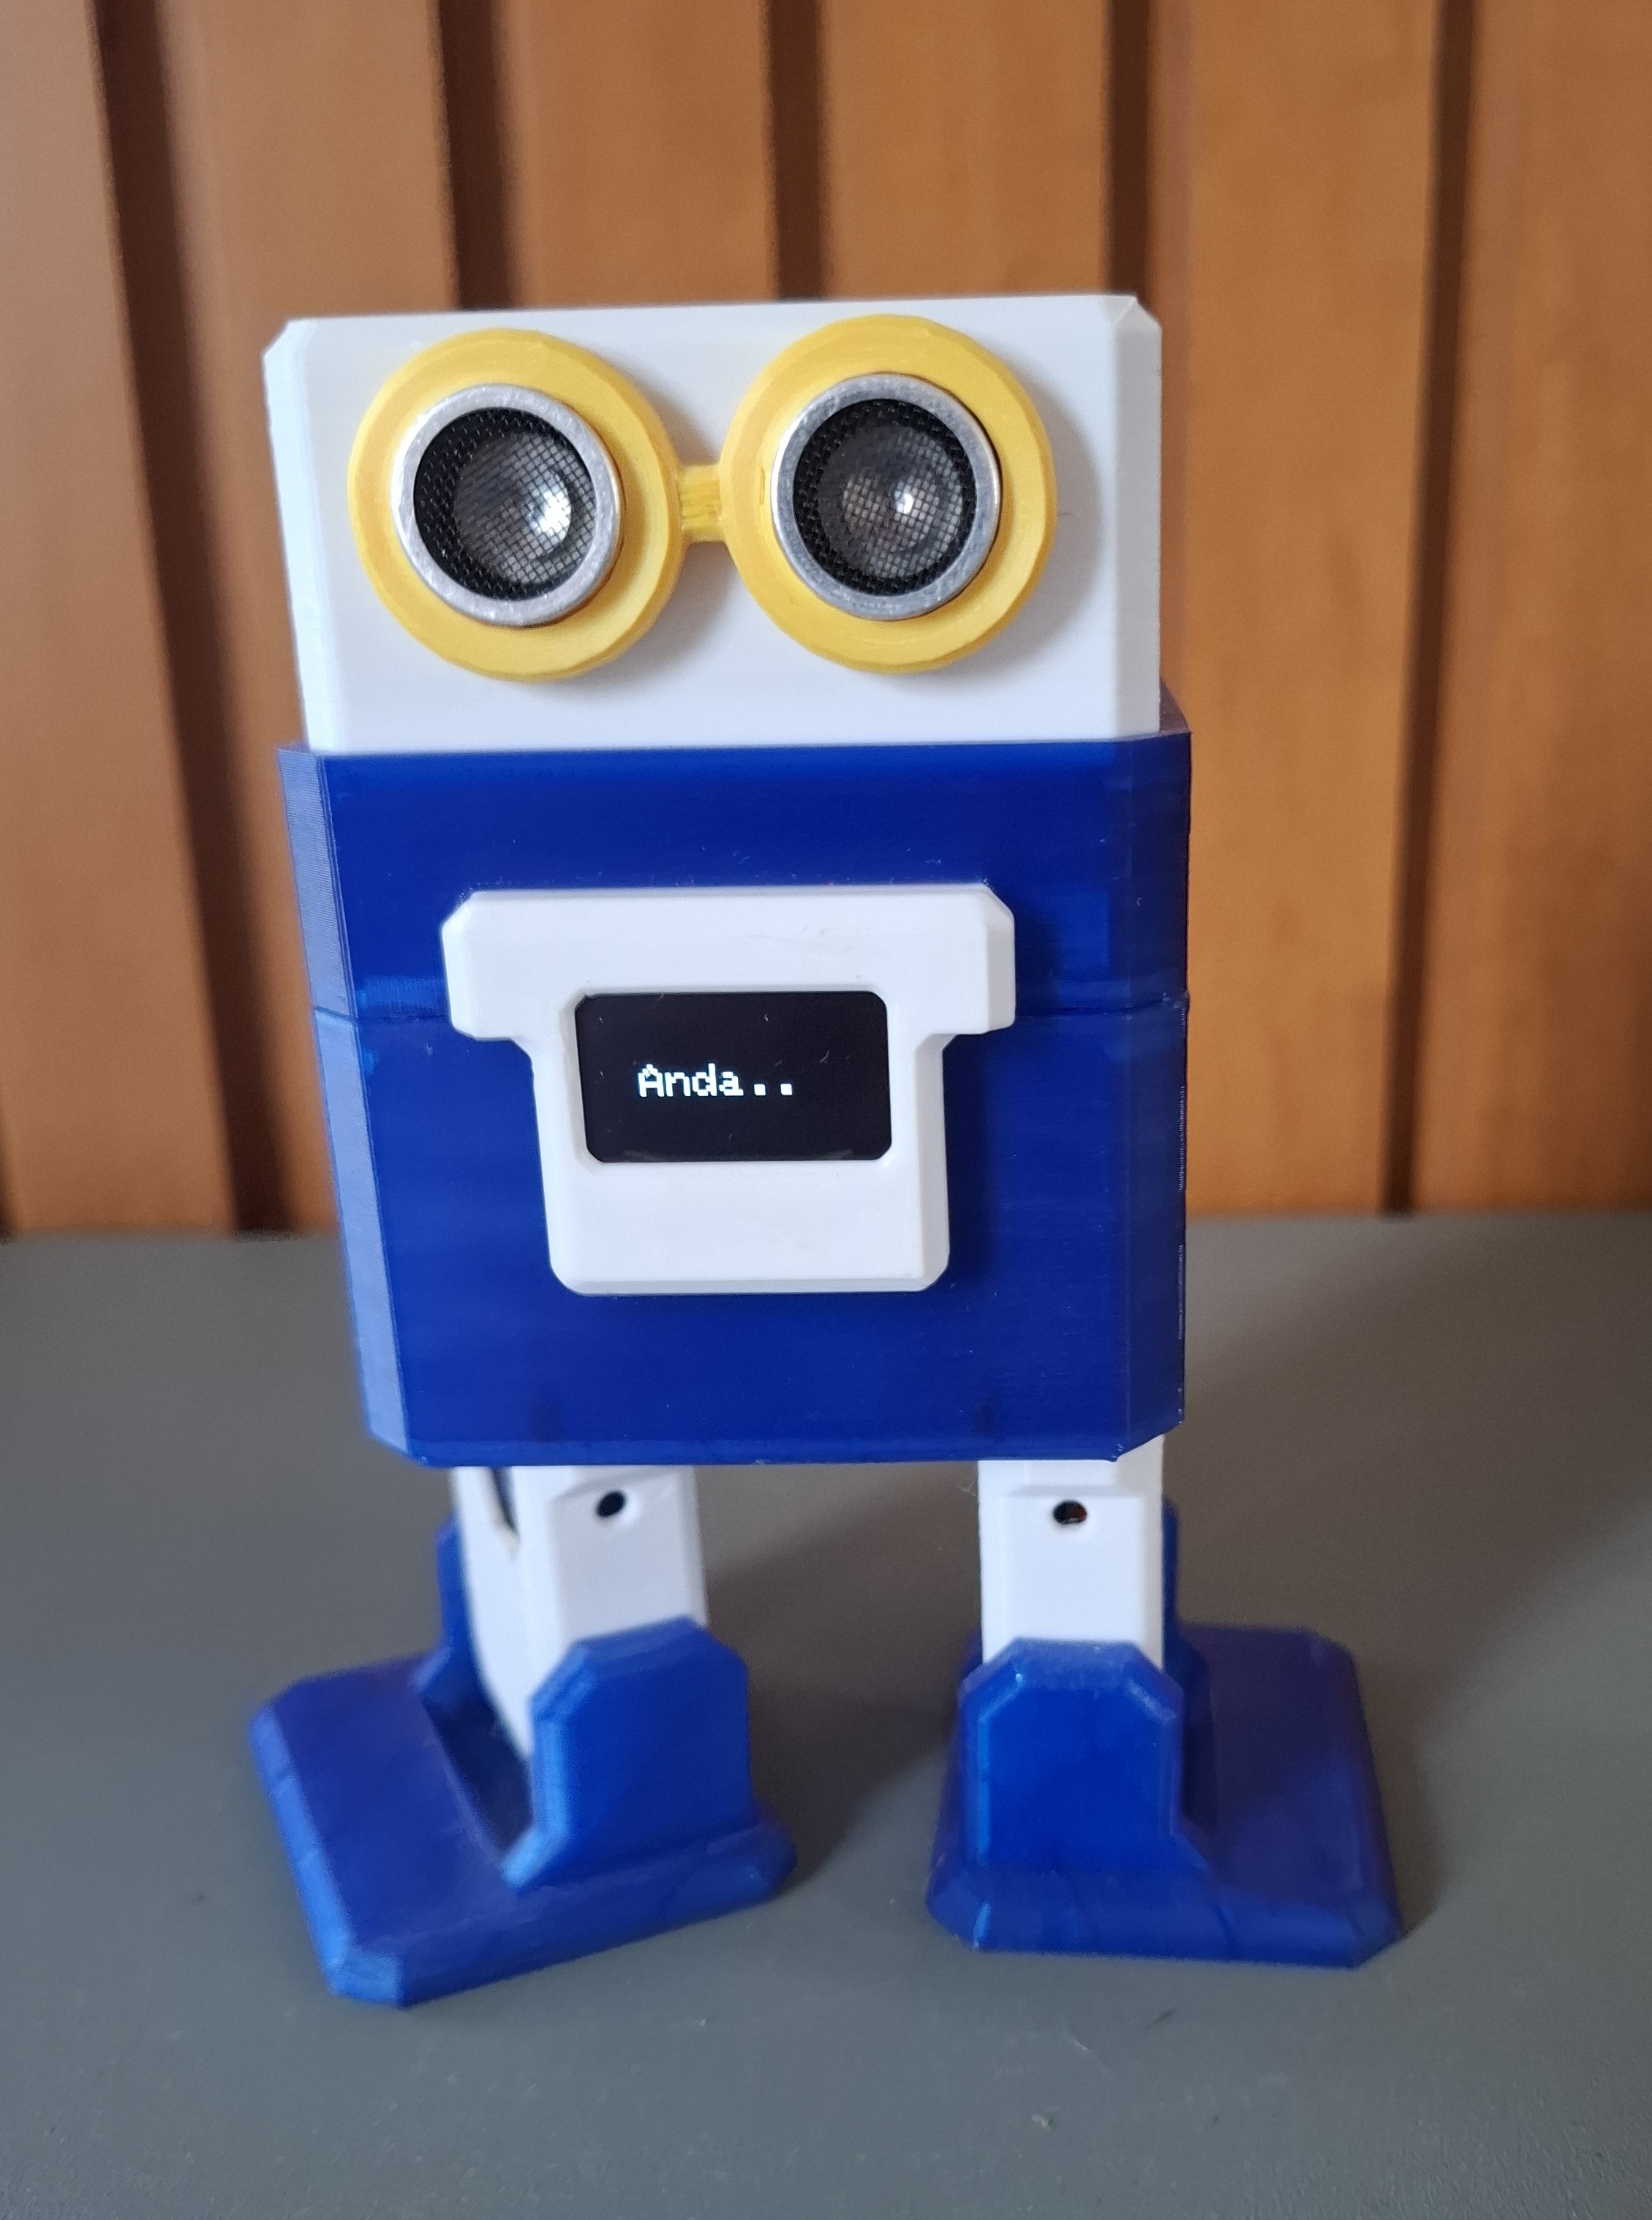
\includegraphics[width=\linewidth]{figures/fig-013b.jpg}
		\subcaption{RoboJoy andando para trás depois de ter um objeto a sua frente.}
	\end{minipage}
	\caption{Detecção de obstáculos com o sensor ultrassônico.}
	\label{fig_ande}
	\source{Autoria Própria.}
\end{minipage}
\end{figure}


\begin{figure}[ht!]
\begin{minipage}{0.75\textwidth}
	\begin{minipage}[t]{0.45\textwidth}
		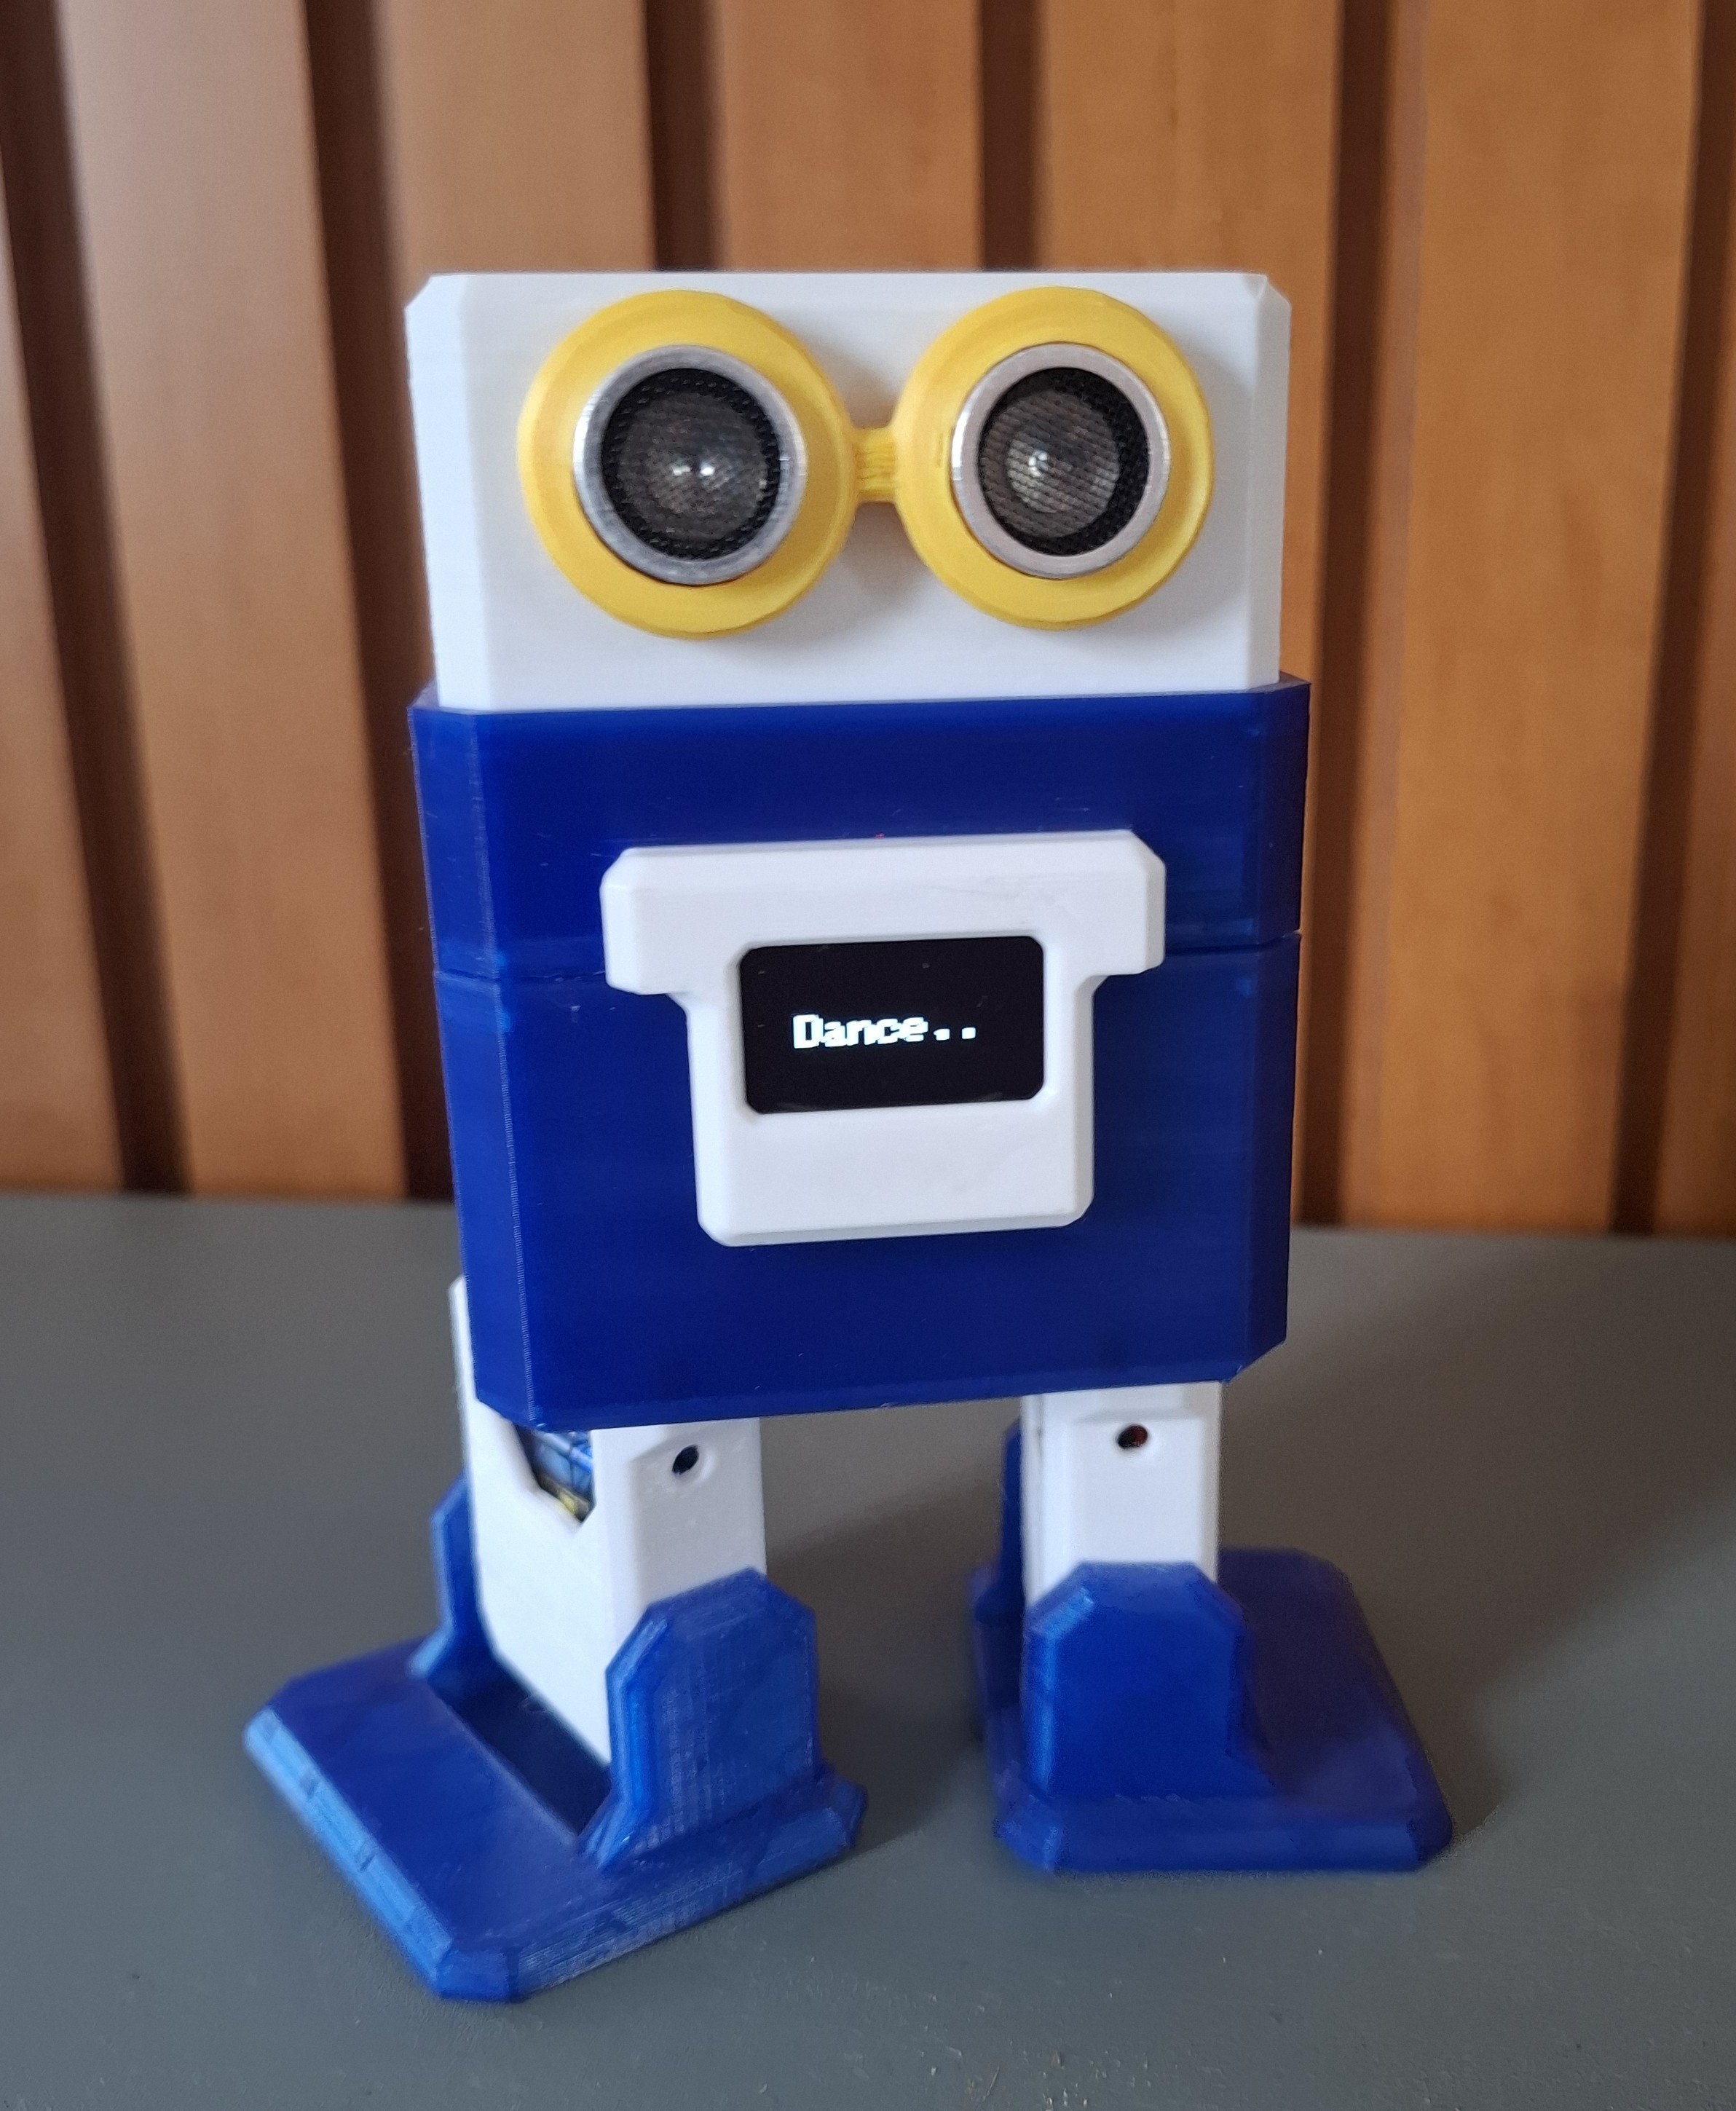
\includegraphics[width=\linewidth]{figures/fig-014a.jpg}
		\subcaption{Dançando com movimentos nos pés.}
	\end{minipage}
	\hfill
	\begin{minipage}[t]{0.40\textwidth}
		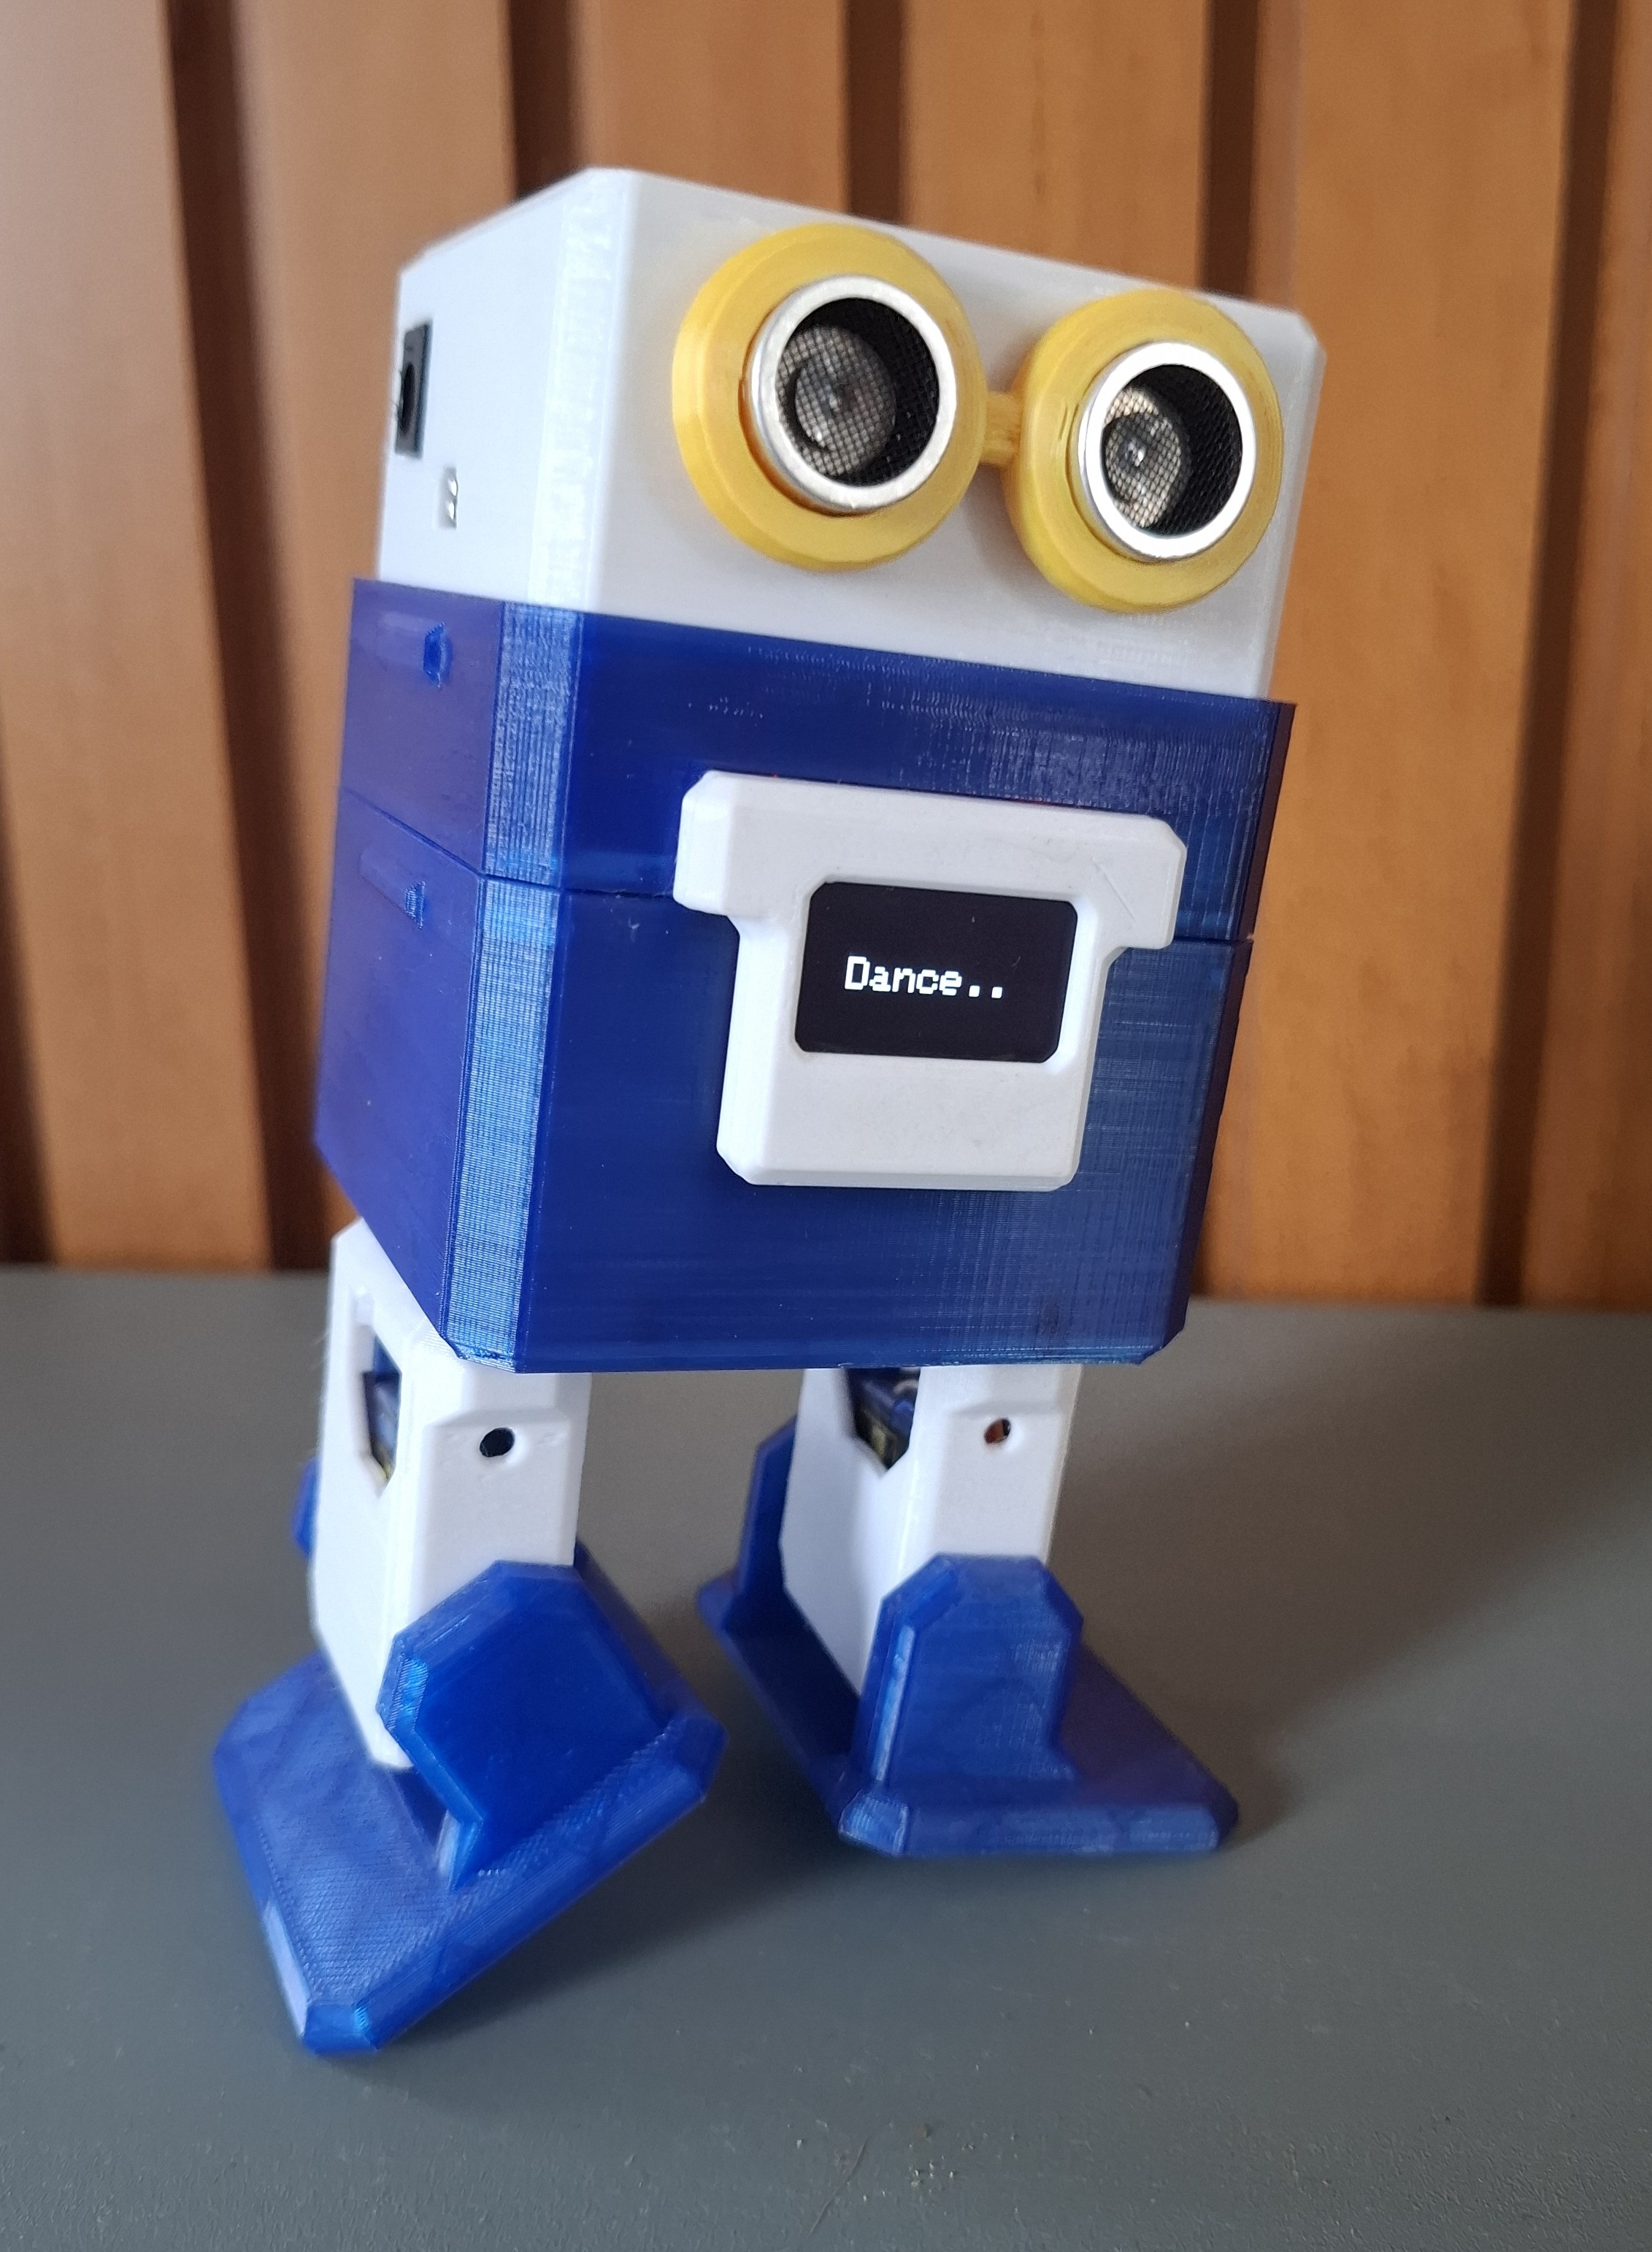
\includegraphics[width=\linewidth]{figures/fig-014b.jpg}
		\subcaption{Dançando com levantamento dos pés.}
	\end{minipage}	
	\caption{Execução da rotina de dança com controle dos servos.}
	\label{fig_dance}
	\source{Autoria Própria.}
\end{minipage}
\end{figure}


\begin{table}[h!]
	\centering
	\caption{Resumo das funções e conceitos aplicados no código do RoboJoy.}
	\label{tab:funcoes_robojoy}
	\resizebox{\textwidth}{!}{
		\begin{tabular}{p{2.6cm}p{3.5cm}p{3.5cm}p{3.5cm}}
			\toprule
			Função & Descrição Técnica & Conceito de Física/Matemática & Objetivo Pedagógico \\
            \midrule
			
			\texttt{smoothMove} &
			Transição gradual entre ângulos dos servomotores, garantindo movimentos suaves e contínuos. &
			Movimento circular e cinemática. &
			Compreender variações de ângulo, tempo e suavização de movimento. \\ \hline
			
			\texttt{ultrasound} &
			Mede a distância por meio de pulsos sonoros refletidos no obstáculo. &
			Ondas sonoras e proporcionalidade. &
			Relacionar tempo de propagação e distância, aplicando proporcionalidade direta. \\ \hline
			
			\texttt{readTemperature} / \texttt{readHumidity} &
			Realiza a leitura de temperatura e umidade do ambiente via sensor DHT11. &
			Termodinâmica e estatística. &
			Coletar e interpretar dados ambientais, organizando-os em gráficos e médias. \\ \hline
			
			\texttt{moveForward} / \texttt{moveBackward} &
			Controle de deslocamento linear do robô para frente e para trás. &
			Movimento linear, velocidade e espaço. &
			Explorar as relações entre tempo, distância e velocidade média. \\ \hline
			
			\texttt{jitter}, \texttt{swing}, \texttt{upDown} &
			Rotinas de dança que coordenam o movimento dos servos. &
			Movimento harmônico e oscilatório. &
			Desenvolver coordenação mecânica e expressão criativa em um contexto lúdico. \\ \hline
			
			\texttt{TelaInicial} &
			Exibe a tela de boas-vindas no display OLED. &
			Comunicação visual e interface digital. &
			Introduzir noções de interface homem-máquina. \\ \hline
			
			\texttt{executarEtapas} &
			Controla o fluxo de ações e etapas do robô conforme interação via toque. &
			Lógica de programação e estruturas condicionais. &
			Compreender algoritmos sequenciais e tomada de decisão. \\ \hline
		\end{tabular}
	}
\end{table}

\newpage
Com o intuito de proporcionar uma melhor visualização das funcionalidades e do desempenho do RoboJoy, foi produzido um vídeo demonstrativo que apresenta as etapas de funcionamento e as respostas do sistema durante a execução das atividades propostas. O vídeo exibe desde a leitura dos sensores até os movimentos coordenados dos servomotores, permitindo observar de forma clara a integração entre \textit{hardware} e \textit{software} explorados no projeto. Para facilitar o acesso, o material foi disponibilizado por meio de um \textit{link} no YouTube e de um código QR (Figura \ref{fig_video}), ambos inseridos neste trabalho, possibilitando que o leitor visualize o resultado final do desenvolvimento e execução do robô em tempo real.


\begin{figure}[ht!]
	\centering
	\begin{minipage}{.30\textwidth}		
\includegraphics[width=\textwidth]{figures/fig-015.jpg}
		\caption{\href{https://youtube.com/shorts/JYWcsW3SlVo}{Vídeo demonstrativo com as etapas do RoboJoy}.}
		\label{fig_video}
		\source{Autoria Própria.}
	\end{minipage}
\end{figure}

A atividade tem como objetivo introduzir o funcionamento completo do sistema RoboJoy, permitindo que os alunos compreendam o ciclo completo de interação entre sensores, atuadores e lógica de programação. Por meio dessa abordagem prática, o estudante assume um papel ativo no processo de aprendizagem, explorando conceitos científicos de forma aplicada.

Sob a ótica da metodologia STEAM, essa atividade:

\begin{itemize}
	\item Promove a integração entre física e matemática (movimento, temperatura, proporções, dados e gráficos);
	\item Estimula o raciocínio lógico e computacional ao analisar o código-fonte e a estrutura condicional das etapas;
	\item Incentiva a criatividade e a expressão artística por meio das rotinas de dança e som;
	\item Reforça o caráter colaborativo e investigativo das metodologias ativas, nas quais o aluno “aprende fazendo” e reflete sobre suas ações.
\end{itemize}

Além disso, o RoboJoy constitui uma ferramenta de aprendizagem tangível, permitindo que o estudante observe, mensure e relacione fenômenos físicos com representações digitais em tempo real. Essa prática favorece o pensamento sistêmico e estimula a curiosidade científica.

Os testes realizados demonstraram funcionamento estável do robô, com leituras coerentes de sensores e boa sincronia entre os servomotores. A integração entre \textit{software} e \textit{hardware} livre se mostrou eficaz, validando a viabilidade do projeto como recurso didático acessível.
O sistema se mostrou modular e expansível, podendo ser adaptado para atividades de coleta de dados experimentais, análise estatística ou simulações de movimento.


\subsection{Elaboração e desenvolvimento das atividades usando o RoboJoy}

As atividades foram elaboradas para promover a integração entre conceitos de física e matemática por meio da robótica educativa, utilizando o robô Otto/RoboJoy, construído com componentes eletrônicos e programado nas plataformas Arduino IDE ou Blockly Otto. Cada atividade foi planejada para estimular a aprendizagem ativa, o raciocínio lógico, a experimentação prática e a interpretação de dados, em alinhamento com a abordagem STEAM.

Durante o processo de desenvolvimento do projeto, verificou-se uma limitação na plataforma Blockly Otto, utilizada para a programação em blocos do robô. Apesar de sua interface intuitiva e do potencial didático para o ensino de lógica e controle de movimentos, a ferramenta não permite a integração simultânea entre a tela OLED e a biblioteca de movimentos do Otto DIY. Essa restrição impede que o robô execute rotinas de movimentação enquanto realiza a exibição de dados no display, como temperatura, umidade ou mensagens programadas.

\subsubsection{Atividade 1 — termodinâmica e ambiente: medindo temperatura e umidade}

\begin{description}
\item[Objetivo:] Compreender os conceitos de temperatura, umidade relativa do ar e sua variação temporal.
\item[Materiais e Métodos:] Sensor utilizado DHT11 (temperatura e umidade) e programação no Blockly Otto ou Arduino IDE.
Os estudantes coletam dados do sensor DHT11 utilizando o código base do Otto modificado para exibir as leituras no display OLED. Durante um intervalo de 30 minutos, registram os valores e constroem (gráficos de variação térmica e umidade) em função do tempo.
\item[Física:] análise de transferência de calor e equilíbrio térmico.
\end{description}

Na etapa de medição de temperatura e umidade, o sensor DHT11 do RoboJoy possibilita a exploração prática dos conceitos de transferência de calor e equilíbrio térmico. Quando o robô é exposto a ambientes com diferentes temperaturas, como um local aquecido e outro ventilado, o sensor registra a variação térmica até atingir uma temperatura de equilíbrio, momento em que não há mais troca líquida de calor entre o sensor e o meio.

A relação entre a quantidade de calor trocada e a variação de temperatura é expressa pela equação fundamental da calorimetria:

% Equação da quantidade de calor
\begin{equation}
	Q = m \cdot c \cdot \Delta T \text{,}
\end{equation}
onde $Q$ é a quantidade de calor ($J$), $m$ é a massa ($kg$), 
$c$ é o calor específico ($J/kg·~^{\circ}\mathrm{C}$) e
$\Delta T $= $T_f$ - $T_i$ (variação de temperatura).

Em uma situação de equilíbrio térmico, quando dois corpos entram em contato e atingem a mesma temperatura final ($T_f$), a soma das trocas de calor é nula:
% Equilíbrio térmico
\begin{equation}
	Q_1 + Q_2 = 0
\end{equation}
% Substituindo pela expressão de calor:
\begin{equation}
	m_1 c_1 (T_f - T_1) + m_2 c_2 (T_f - T_2) = 0
\end{equation}

Com base nesses conceitos, os estudantes podem correlacionar as leituras reais do sensor DHT11 com o processo de troca de energia térmica, compreendendo que o equilíbrio é atingido quando as leituras se estabilizam no display OLED do robô.

\begin{description}
    \item[Matemática:] interpretação de gráficos e medidas estatísticas (média e desvio padrão).
\end{description}

As leituras obtidas pelo sensor (temperatura e umidade) também permitem desenvolver competências matemáticas relacionadas à interpretação de dados experimentais. Após coletar um conjunto de medições em diferentes momentos, é possível calcular medidas estatísticas e representar graficamente os resultados.

A média aritmética das medidas é dada por:
% Média aritmética das medições
\begin{equation}
	\bar{x} = \frac{1}{n} \sum_{i=1}^{n} x_i \text{,}
\end{equation}
onde $x_i$ representa cada valor observado; $n$ é o número total de observações.

Para avaliar a dispersão dos dados, utiliza-se o desvio padrão, que indica o quanto as medições variam em torno da média:

% Desvio padrão das medições
\begin{equation}
	s = \sqrt{\frac{1}{n-1} \sum_{i=1}^{n} (x_i - \bar{x})^2} .
\end{equation}

Essas expressões permitem que os estudantes interpretem o comportamento das variáveis medidas pelo RoboJoy, identificando a precisão do sensor e a influência de fatores ambientais (como correntes de ar ou variação de umidade) sobre os resultados.

Por fim, os dados podem ser apresentados em gráficos de linha ou dispersão, relacionando tempo (eixo x) e temperatura ou umidade (eixo y), de modo a visualizar tendências, variações e situações de equilíbrio.

\textbf{Extensão STEAM:} discussão sobre o papel da temperatura em sistemas eletrônicos e sustentabilidade ambiental.


\subsubsection{Atividade 2 — ondas sonoras e movimento (sensor ultrassônico)}

\begin{description}
    \item[Objetivo:] Relacionar o tempo de resposta do sensor com a velocidade do som no ar.
    \item[Materiais e Métodos:] Sensor utilizado HC-SR04 e programação no Blockly Otto (modo distância) ou código Arduino com `pulseIn()`.
    \item[Descrição:] Os estudantes posicionam o robô diante de superfícies a diferentes distâncias e analisam o tempo de resposta registrado. Com base nos dados, calculam a velocidade do som e comparam com o valor teórico (343 m/s).
    \item[Física:] ondas mecânicas, reflexão e propagação.
\end{description}


Nesta atividade, o sensor ultrassônico do RoboJoy foi utilizado para medir a distância até obstáculos, permitindo discutir conceitos de ondas mecânicas, especialmente reflexão e propagação sonora.

O sensor funciona emitindo uma onda sonora de alta frequência (ultrassom), que se propaga no ar, reflete em um objeto e retorna ao receptor. O tempo entre o envio e o retorno da onda é usado para calcular a distância percorrida.

A relação entre a velocidade da onda, o tempo e a distância é dada por:
\begin{equation}
	v = \frac{2d}{\Delta t} \text{,}
\end{equation}
onde $v$ é a velocidade do som no ar (aproximadamente 340~$\mathrm{m/s}$);
$d$ é a distância entre o sensor e o obstáculo (em metros);
$\Delta t$ é o tempo total medido entre a emissão e a recepção do pulso (em segundos); e o fator 2 aparece porque o som percorre o trajeto de ida e volta.

Esse experimento permite observar que a reflexão da onda sonora ocorre quando ela encontra uma superfície, retornando ao emissor. A variação do tempo de retorno indica a mudança de posição do obstáculo, podendo ser correlacionada com o conceito de propagação das ondas em diferentes meios.

Além disso, os estudantes podem discutir como fatores ambientais, como temperatura e umidade, afetam a velocidade do som, utilizando a aproximação empírica:

\begin{equation}
	v_{\text{som}} = 331 + 0.6 \cdot T ,
\end{equation}
onde $T$ é a temperatura do ar em ($^{\circ}\mathrm{C}$).

Essa equação mostra que o som se propaga mais rapidamente em temperaturas mais elevadas, o que pode ser explorado comparando leituras do sensor em ambientes de diferentes condições térmicas.

\textbf{Matemática:} proporcionalidade e função linear (tempo × distância).

A análise das medições realizadas pelo sensor ultrassônico possibilita a aplicação de conceitos matemáticos de proporcionalidade direta e função linear.

Quando o sensor registra a variação do tempo de resposta conforme a distância do obstáculo, os dados podem ser organizados em pares ordenados ($t, d$), permitindo construir um gráfico da distância em função do tempo.

A relação é linear e pode ser expressa pela equação da função do primeiro grau:

\begin{equation}
	d = \frac{v}{2} \cdot t \text{,}
\end{equation}
onde $d$ é a distância medida (em metros);
$v$ é a velocidade do som (em m/s);
$t$ é o tempo medido (em segundos); e
o fator $\frac{1}{2}$ corresponde ao percurso de ida e volta do pulso ultrassônico.

Dessa forma, o gráfico distância × tempo deve apresentar um comportamento linear, cujo coeficiente angular (inclinação) é diretamente proporcional à velocidade da onda sonora.

A partir disso, os alunos podem discutir funções lineares, taxas de variação, e até análise de erros experimentais.

\begin{description}
    \item[Extensão STEAM:] visualização gráfica no computador e debate sobre sensores em automóveis e sistemas de segurança.
\end{description}


\subsubsection{Atividade 3 — cinemática e movimento circular (servomotores)}

\begin{description}
    \item[Objetivo:] Explorar o movimento angular e o conceito de velocidade e aceleração angular.
    \item[Materiais e Métodos:] 4 servomotores SG90 e programação no Blockly Otto (modo dança) ou código Arduino usando `servo.write()`.
    \item[Descrição:] Os estudantes programam o RoboJoy para realizar uma sequência de movimentos circulares com ângulos definidos, registrando os valores de ângulo ($\theta$), tempo ($t$) e posição para construir uma tabela experimental. A partir desses dados, calculam a velocidade angular ($\omega$). Essa abordagem permite comparar os valores teóricos e experimentais, reforçando o aprendizado interdisciplinar entre física e matemática.Física:
    \item[Física:] movimento circular uniforme.
\end{description}

Nesta atividade, o RoboJoy foi programado para executar movimentos circulares uniformes com seus servomotores, representando o comportamento de um corpo que gira em torno de um eixo com velocidade angular constante. Cada servo realiza rotações controladas em ângulos pré-definidos, possibilitando observar como a posição angular varia com o tempo. O conceito fundamental que descreve esse movimento é a posição angular, expressa por:

\begin{equation}
	\theta(t) = \theta_0 + \omega \cdot t \text{,}
\end{equation}
onde $\theta(t)$ é a posição angular no instante ($t$) (em rad),
$\theta_0$ é a posição inicial,
$\omega$ é a velocidade angular (em rad/s) e $t$ é o tempo decorrido.

A velocidade angular relaciona o ângulo percorrido e o intervalo de tempo da rotação:
\begin{equation}
	\omega = \frac{\Delta \theta}{\Delta t} .
\end{equation}

Em um movimento circular uniforme (MCU), ($\omega$) permanece constante, o que significa que o servo percorre ângulos iguais em tempos iguais. Essa regularidade permite aos estudantes analisarem a periodicidade e compreenderem o comportamento rotacional em sistemas reais, como rodas, motores e engrenagens.

\begin{description}
    \item[Matemática:] funções trigonométricas aplicadas à rotação.
\end{description}

A análise matemática do movimento circular permite relacionar a posição angular do servo com as funções trigonométricas seno e cosseno, representando o deslocamento da extremidade do braço (ou perna) do robô no plano cartesiano.
Considerando o raio ($r$) da trajetória circular, as posições $x$ e $y$ podem ser determinadas pelas equações:

\begin{equation}
	x = r \cdot \cos(\theta) ,
\end{equation}
\begin{equation}
	y = r \cdot \sin(\theta) \text{,}
\end{equation}
onde $x$ e $y$ representam as coordenadas do ponto em movimento,
$r$ é o raio do círculo (distância do eixo até a extremidade) e
$\theta$ é o ângulo em radianos.

Essas funções descrevem o movimento periódico característico das rotações, permitindo representar graficamente o comportamento oscilatório dos servos. Assim, os estudantes relacionam a teoria das funções trigonométricas com o movimento físico real do robô, observando que o gráfico de $x(t)$ e $y(t)$ segue o formato de ondas senoidais.

\begin{description}
    \item[Extensão STEAM:] simulação de articulações humanas e uso de servos em engenharia.
\end{description} 


\subsubsection{Atividade 4 — estatística e gráficos (análise de dados dos sensores)}

\begin{description}
    \item[Objetivo:]  Coletar dados ambientais e de distância para análise estatística.
    \item[Materiais e Métodos:] Sensores utilizados display OLED, DHT11 e HC-SR04, e programação no Arduino IDE ou no Blockly Otto.
    \item[Descrição:] Os estudantes registram 20 leituras de temperatura, umidade e distância em diferentes momentos. Com os dados, calculam a média, mediana, moda e variância. Depois criam os gráficos no \textit{software} livre (LibreOffice Calc).
    \item[Física:] análise experimental e variáveis ambientais.
\end{description}

Do ponto de vista físico, os sensores do RoboJoy possibilitam o estudo das variáveis ambientais que afetam a medição como: temperatura do ambiente, umidade e obstáculos próximos. Durante o experimento, observa-se que pequenas variações nas condições do ambiente (correntes de ar, presença humana, fontes de calor) influenciam diretamente as leituras dos sensores, reforçando o conceito de grandezas físicas variáveis e a necessidade de controle experimental.

A análise dos dados permite aos estudantes compreender que todo instrumento de medição possui incertezas, e que a repetição de medições melhora a precisão dos resultados. Essa reflexão aproxima o experimento escolar dos métodos científicos reais, onde a observação e o registro sistemático de dados são essenciais para validar os resultados.

O objetivo é compreender a variação das grandezas temperatura ($T$), umidade ($U)$ e distância ($d$) em função do tempo, representando a coleta de dados experimentais. A variação de uma grandeza física no tempo, pode ser calculada:

\begin{equation}
	\Delta X = X_f - X_i \text{,}
\end{equation}
onde $\Delta X$ representa a grandeza medida (temperatura, umidade ou distância);
$X_i$ é o valor inicial e
$X_f$ é o valor final.

Essa variação é usada para identificar tendências de aumento ou diminuição ao longo do tempo. A taxa de variação (ou gradiente temporal) é encontrada:
\begin{equation}
	\frac{\Delta X}{\Delta t} = \frac{X_f - X_i}{t_f - t_i} .
\end{equation}

Essa relação permite analisar a rapidez da variação de temperatura, umidade ou distância entre dois instantes, o conceito físico relacionado à taxa de mudança e estabilidade do sistema.

\begin{description}
    \item[Matemática:] estatística descritiva e visualização de dados.
\end{description}

A etapa matemática envolve o tratamento dos dados experimentais com base nos conceitos de estatística descritiva. Os estudantes aplicam fórmulas para calcular a média, mediana, moda e variância, avaliando a consistência das medições e a presença de possíveis erros experimentais. As principais equações utilizadas são:

Média aritmética:
\begin{equation}
	\bar{x} = \frac{1}{n} \sum_{i=1}^{n} x_i \text{,}
\end{equation}
onde $\bar{x}$ é a média dos valores medidos; $n$ é o número total de observações e $x_i$ é o valor da $i$-ésima observação. 

A média fornece uma visão geral do comportamento médio do sensor ao longo do experimento.

Mediana:
\begin{equation}
	\tilde{x} =
	\begin{cases}
		x_{\frac{n+1}{2}} & \text{, se } n \text{ for ímpar} \\
		\frac{x_{\frac{n}{2}} + x_{\frac{n}{2}+1}}{2} & \text{, se } n \text{ for par.}
	\end{cases}
\end{equation}

A mediana indica o valor central dos dados e é útil quando há valores extremos nas medições.

Moda:
\begin{equation}
	Mo = \text{valor de } x_i \text{ com maior frequência.}
\end{equation}

A moda mostra qual valor ocorre com maior frequência entre as leituras, sendo útil para identificar padrões repetitivos nas medições do sensor.

Variância amostral:
\begin{equation}
	s^2 = \frac{1}{n-1} \sum_{i=1}^{n} (x_i - \bar{x})^2 .
\end{equation}

A variância mede o grau de dispersão dos dados em torno da média. Quanto maior $s^2$, mais os valores se afastam do valor médio.

Desvio padrão:
\begin{equation}
	s = \sqrt{\frac{1}{n-1} \sum_{i=1}^{n} (x_i - \bar{x})^2} .
\end{equation}

O desvio padrão $s$ expressa a dispersão média das medidas em relação à média. Em física experimental, ele representa a precisão do instrumento de medição.

Erro percentual experimental:
\begin{equation}
	E(\%) = \left| \frac{x_{\text{exp}} - x_{\text{ref}}}{x_{\text{ref}}} \right| \times 100 \text{,}
\end{equation}
onde
$x_{\text{exp}}$ é o valor medido pelo sensor e
$x_{\text{ref}}$ é o valor de referência (por exemplo, de um termômetro digital externo). 

Essa equação é opcional, mas ideal para comparar a precisão do RoboJoy com instrumentos convencionais.

Representação gráfica (modelo linear):
\begin{equation}
	y = a \cdot t + b \text{,}
\end{equation}
onde $y$ é a grandeza observada (temperatura, umidade, distância); 
$t$ é o tempo; 
$a$ é o coeficiente angular (taxa de variação da grandeza) e 
$b$ é o valor inicial da grandeza. 

Esse modelo permite verificar se a variação é constante (linear) ou apresenta oscilações ao longo do tempo. Após os cálculos, os estudantes representam graficamente as grandezas medidas ao longo do tempo ou das condições ambientais, interpretando visualmente tendências, picos e estabilizações. Esses gráficos permitem verificar, por exemplo, a estabilidade térmica do ambiente, a relação entre umidade e temperatura, ou a precisão do sensor ultrassônico em diferentes distâncias.

\begin{description}
    \item[Extensão STEAM:] introdução à análise de dados em sistemas inteligentes (IoT).
\end{description}

\subsubsection{Atividade 5 — trigonometria e funções (movimento dos servos)}

\begin{description}
    \item[Objetivo:] Relacionar o ângulo de movimento dos servos com funções trigonométricas.
    \item[Materiais e Métodos:] Servomotores e programação no Blockly Otto.
    \item[Descrição:] Os estudantes programam o RoboJoy para movimentar seus pés e pernas de forma coordenada, medindo o deslocamento resultante em função do ângulo de rotação.
    \item[Física:] movimento harmônico simples e amplitude.
\end{description}

O movimento oscilatório realizado pelo RoboJoy pode ser interpretado como um exemplo de Movimento Harmônico Simples (MHS), no qual a posição do corpo varia periodicamente em torno de um ponto de equilíbrio. A posição em função do tempo é dada por:

\begin{equation}
	x(t) = A \cdot \sin(\omega t + \varphi) \text{,}
\end{equation}
onde $x(t)$ é a posição do robô em função do tempo; 
$A$ é a amplitude do movimento (máximo deslocamento em relação ao ponto de equilíbrio); 
$\omega$ é a frequência angular, em rad/s; 
$t$ é o tempo (s) e
$\varphi$ é a fase inicial (rad).

A velocidade e a aceleração instantâneas podem ser obtidas pelas derivadas sucessivas da função posição:
\begin{equation}
	v(t) = \frac{dx}{dt} = A \omega \cos(\omega t + \varphi) ,
\end{equation}
\begin{equation}
	a(t) = \frac{d^2x}{dt^2} = -A \omega^2 \sin(\omega t + \varphi) .
\end{equation}

O sinal negativo na aceleração indica que ela atua sempre em direção ao ponto de equilíbrio, característica fundamental do MHS.

A relação entre a frequência angular e o período do movimento é dada por:
\begin{equation}
	\omega = \frac{2\pi}{T} \text{,}
\end{equation}
onde
$T$ é o período (tempo necessário para completar uma oscilação completa).

\begin{description}
    \item[Matemática:] seno, cosseno e relação entre ângulo e deslocamento.
\end{description}

O movimento harmônico simples é descrito por funções trigonométricas. O deslocamento, a velocidade e a aceleração são funções do ângulo $\theta = \omega t + \varphi$, obedecendo às relações:
\begin{align}
	x(t) &= A \sin(\theta), \\
	v(t) &= A \omega \cos(\theta),\\
	a(t) &= -A \omega^2 \sin(\theta).
\end{align}

A função seno representa o deslocamento oscilatório, enquanto o cosseno descreve a variação da velocidade ao longo do tempo. O uso das funções trigonométricas permite relacionar o ângulo de rotação dos servos do RoboJoy com o deslocamento linear das suas pernas durante o movimento oscilatório.

\begin{description}
    \item[Extensão STEAM:] representação gráfica das funções e sua aplicação no controle de movimentos robóticos.
\end{description}

\subsubsection{Atividade 6 — funções lineares e proporcionalidade (distância × ação)}

\begin{description}
    \item[Objetivo:] Entender a relação linear entre a distância detectada e o movimento do robô.
    \item[Materiais e Métodos:] sensores utilizados ultrassônico e servomotores, e programação no Blockly Otto (modo reativo).
    \item[Descrição:] Os estudantes configuram o RoboJoy para “reagir” à aproximação de objetos: quanto menor a distância, maior a velocidade do movimento ou o ângulo de resposta.
    \item[Física:] resposta proporcional e retroalimentação de sistemas.
\end{description}

O RoboJoy pode ser programado para responder de forma proporcional a estímulos externos, por exemplo, alterar sua distância em relação a um obstáculo medido pelo sensor ultrassônico. Esse tipo de comportamento pode ser descrito fisicamente como um sistema com retroalimentação (\textit{feedback}) e resposta proporcional, muito comum em sistemas de controle automático.

A variável de saída (ação do robô) depende linearmente do erro entre o valor medido e o valor de referência desejado. Essa relação é descrita por:

\begin{equation}
	A(t) = K_p \cdot e(t) \text{,}
\end{equation}
onde
$A(t)$ é a ação de controle (por exemplo, rotação do servo ou deslocamento do robô); 
$K_p$ é a constante de proporcionalidade (ganho do sistema) e
$e(t)$ é o erro instantâneo, definido como a diferença entre o valor de referência e o valor medido: 
\begin{equation}
	e(t) = x_{\text{ref}} - x(t) .
\end{equation}

Quando $e(t)$ tende a zero, o sistema se estabiliza, caracterizando o equilíbrio dinâmico obtido pela retroalimentação proporcional.

\begin{description}
    \item[Matemática:]  funções lineares e coeficiente angular.
\end{description}

Do ponto de vista matemático, a resposta proporcional do sistema pode ser representada por uma função linear da forma:
\begin{equation}
	y = a \cdot x + b \text{,}
\end{equation}
onde
$y$ é a variável dependente (ação ou resposta do robô); 
$x$ é a variável independente (erro ou estímulo medido);
$a$ é o coeficiente angular, que representa a taxa de variação entre as duas grandezas (equivalente ao ganho $K_p$) e
$b$ é o coeficiente linear, indicando o valor inicial da função (quando $x = 0$).

O coeficiente angular pode ser determinado pela relação:
\begin{equation}
	a = \frac{\Delta y}{\Delta x} .
\end{equation}

Assim, os estudantes podem comparar experimentalmente como diferentes valores de ganho $K_p$ influenciam a rapidez e a estabilidade do movimento do robô, visualizando graficamente a proporcionalidade entre erro e resposta do sistema.

\begin{description}
    \item[Extensão STEAM:] analogia com sensores de proximidade em robôs autônomos e veículos inteligentes.
\end{description}



\subsection{Discussões}

As atividades desenvolvidas possibilitam aos estudantes compreender conceitos abstratos de física e matemática por meio da prática, promovendo o desenvolvimento de habilidades de programação, medição, análise e raciocínio científico. A utilização combinada do Blockly Otto (ambiente de programação visual e intuitivo) e do Arduino IDE (ambiente textual e analítico) ampliou o alcance da proposta, atendendo diferentes estilos de aprendizagem e reforçando o caráter inclusivo, criativo e investigativo da metodologia.

Durante a realização das atividades, prevê-se que, os estudantes apresentem alto nível de colaboração e participação, demonstrando curiosidade, iniciativa e cooperação em todas as etapas. A metodologia baseada em aprendizagem por projetos e prática deverá favorecer a formulação de teorias, o teste de soluções e a reflexão sobre os resultados obtidos, estimula o protagonismo estudantil e a construção ativa do conhecimento.

Do ponto de vista técnico, identificou-se um conflito entre as bibliotecas utilizadas no ambiente Blockly Otto, especificamente entre a biblioteca da tela OLED e a biblioteca de movimentos do Otto DIY. Esse conflito impede a execução simultânea de exibição de informações no display e das rotinas de dança quando programado no Blockly. Assim, para integrar essas duas funções no RoboJoy, foi necessário desenvolver a programação diretamente no Arduino IDE para a criação do RoboJoy original. Nesse ambiente, a gestão das bibliotecas é mais flexível, permitindo que o robô execute as danças enquanto exibe dados de sensores no display OLED.

Essa situação será explorada pedagogicamente como parte do processo de aprendizagem, possibilitando que os estudantes compreendam as diferenças entre linguagens visuais e textuais, bem como as limitações de compatibilidade entre bibliotecas. Espera-se que a transição para o Arduino IDE incentive a autonomia técnica e o pensamento computacional, estimulando a resolução de problemas de forma criativa e fundamentada.

Entre os desafios observados, destacam-se:
\begin{itemize}
	\item a dificuldade inicial de integração entre \textit{hardware} e \textit{software}, exigindo tempo adicional para calibração e testes;
	\item a limitação da tela OLED quanto à exibição simultânea de múltiplas variáveis;
	\item e a necessidade de aprofundar a análise quantitativa dos dados obtidos, fortalecendo a dimensão científica das atividades.
\end{itemize}

Mesmo diante dessas limitações, os resultados qualitativos indicam o potencial pedagógico da abordagem. A prática com o RoboJoy aproximou os conteúdos de física e matemática da realidade tecnológica cotidiana, possibilitando a compreensão de conceitos como transferência de energia, movimento, funções e estatística de forma mais concreta e contextualizada.

Os resultados reforçam o caráter interdisciplinar e integrador da abordagem STEAM, evidenciando que a robótica pedagógica livre é um recurso fundamental para o ensino de ciências. O trabalho com o Otto DIY e suas adaptações promove o raciocínio lógico, a criatividade e a autonomia, consolidando uma aprendizagem significativa e alinhada às metodologias ativas contemporâneas.



\section{Considerações finais}\label{sec-conclusoes}

O presente trabalho apresentou uma proposta de integração entre Robótica Educacional Livre e o ensino de física e matemática, utilizando o robô RoboJoy, desenvolvido a partir do modelo Otto DIY. A metodologia proposta fundamentou-se nos princípios das metodologias ativas e da abordagem STEAM (Ciência, Tecnologia, Engenharia, Artes e Matemática), favorecendo a aprendizagem significativa por meio da prática (experimentação), da criação e da resolução de problemas.

A elaboração das atividades pedagógicas com o RoboJoy visa promover a compreensão de conceitos científicos e matemáticos por meio da prática, explorando grandezas físicas, análise de dados e modelagem matemática associadas a situações reais mediadas pela tecnologia. A interação entre \textit{hardware} e \textit{software} estimula o pensamento lógico e a autonomia intelectual dos estudantes, que se tornam protagonistas do próprio processo de aprendizagem.

Espera-se que a implementação das atividades contribua para o trabalho em equipe dos estudantes e para o desenvolvimento de competências relacionadas à inovação, colaboração e pensamento crítico. Além disso, a proposta aproxima o ensino de ciências do cotidiano tecnológico, ampliando as possibilidades de inclusão digital e equidade educacional.

O projeto evidenciou a importância de compreender as limitações de compatibilidade entre bibliotecas e ambientes de programação, destacando a necessidade de utilizar o Arduino IDE para integrar a tela OLED com os movimentos do robô. Essa reflexão sobre o processo de desenvolvimento tecnológico é, por si só, uma oportunidade formativa relevante para professores e estudantes, pois estimula a resolução de problemas e o raciocínio computacional.

Os resultados esperados e as aplicações futuras desta proposta dialogam diretamente com os Objetivos de Desenvolvimento Sustentável (ODS), em especial com o ODS 4 — Educação de Qualidade, o ODS 9 — Indústria, Inovação e Infraestrutura, e o ODS 10 — Redução das Desigualdades. Ao promover o acesso a tecnologias abertas, o projeto contribui para uma educação mais inclusiva, criativa e equitativa.

Por fim, o RoboJoy representa não apenas um recurso tecnológico, mas um instrumento de transformação educacional que democratiza o acesso à ciência, à engenharia e à programação, fortalecendo a formação de cidadãos críticos e inovadores capazes de atuar de forma consciente e sustentável na sociedade contemporânea.


\printbibliography\label{sec-bib}
% if the text is not in Portuguese, it might be necessary to use the code below instead to print the correct ABNT abbreviations [s.n.], [s.l.]
%\begin{portuguese}
%\printbibliography[title={Bibliography}]
%\end{portuguese}
%\bibliographystyle{apalike}% ou outro .bst, dependendo da exigência
%\fontsize{11}{0}\selectfont\bibliography{article}

\begin{funding}
A autora agradece ao Fundo de Desenvolvimento Acadêmico (FDA) da Universidade Federal do Paraná (UFPR), à Fundação Araucária (FA) e à Secretaria de Estado da Ciência, Tecnologia e Ensino Superior do Paraná (SETI) pelo apoio financeiro destinado ao desenvolvimento desta pesquisa.
\end{funding}

\begin{dataavailability}
\txtdataavailability{databody} % options: dataavailable, dataonly, databody, datanotav, nodata
\end{dataavailability}


\end{document}

